\documentclass[12pt]{article}
\usepackage{natbib}
\usepackage[]{hyperref}
\usepackage{bm}
\usepackage{amsfonts}
\usepackage{graphicx}


\oddsidemargin 0.0mm
\evensidemargin 0.0mm
\textwidth 160mm
\topmargin -10mm
\textheight 230mm
% \pagestyle{empty}

%%%%%%%%%%%%%%%%%%%%%%%%%%%%%%%%%%%%%%%%%%%%%%%%%%%%%%%%%%%%%%%%%%%

\newcommand{\threej}[6]
{ \left(\begin{array}{ccc}
#1&#2&#3\\
#4&#5&#6
\end{array}\right) }

\newcommand{\sixj}[6]
{ \left\{\begin{array}{ccc}
#1&#2&#3\\
#4&#5&#6
\end{array}\right\} }

\def\separation {0.5cm}
\def\non{\nonumber \\}
\def\DnuD     {\hbox{$\Delta\nu_D$}}
\def\Jbar     {\hbox{$\bar J$}}
\def\j        {\hbox{$\jmath$}}
\def\N        {\hbox{$\cal N$}}
\def\Ie       {\hbox{$I_e$}}
\def\Ji       {\hbox{$\bar J^i_\mathrm{ext}$}}
\def\about    {\hbox{$\sim$}}
\def\x        {\hbox{$\times$}}
\def\half     {\hbox{$1\over2$}}
\def\Ncr      {\hbox{$N'_{\rm cr}$}}
\def\mic      {\hbox{$\mu$m}}
\def\ion#1#2  {#1\,{\small {#2}} }
\def\tot      {\tau_t}
\def\t(#1){\tau^{#1}}
\def\a(#1){\alpha^{#1}}
\def\H{\textsc{Hazel}}
\def\HM{\textsc{P-Hazel}}
\def\LVG      {\texttt{LVG}}
\def\slab     {\texttt{slab}}

%%%%%%%%%%%%%%%%%%%%%%%%%%%%%%%%%%%%%%%%%%%%%%%%%%%%%%%%%%%%%%%%%%%


% For generation of the HTML manual with tth:
\def\tthdump#1{#1}      % For generating TeX source; ignored by tth
% Redefine symbols problematic for the browser:
%%tth:\def\ga{\hbox{$>\sim$}}
%%tth:\def\la{\hbox{$<\sim$}}
%%tth:\def\Mo{\hbox{$M_o$}}
%%tth:\def\Lo{\hbox{$L_o$}}
%%tth:\def\Mdot{\hbox{$M^{dot}$}}
%%tth:\def\Ivezic{Ivezic}

%%tth:\begin{html}<TITLE>User Manual for MOLPOP-CEP</TITLE>\end{html}
%%tth: This HTML file was generated from the TeX source by
%%tth: the translator TTH, which uses symbol fonts.  These fonts are
%%tth: not normally enabled for Netscape running under X, because of
%%tth: the way Netscape groups its fonts. If your browser has problems
%%tth: displaying the math symbols in this manual, an easy fix can be found
%%tth: on the TTH website at
%%tth:\begin{html}<A HREF="http://hutchinson.belmont.ma.us/tth/Xfonts.html">http://hutchinson.belmont.ma.us/tth/Xfonts.html</A>\end{html}
%%tth:\begin{html}<HR>\end{html}
%%%%%%%%%%%%%%%%%%%%%%%%%%%%%%%%%%%%%%%%%%%%%%%%%%%%%%%%%%%%%%%%%%%

\begin{document}

\title                  {\sc User Manual for \H\ and \HM\footnote{\H\ (an acronym for HAnle and ZEeman Light) is one of the IAC computer
programs for the synthesis and inversion of Stokes profiles resulting from the joint action of the Hanle and Zeeman effects.}}

\author{ A. Asensio Ramos \\
         Instituto de Astrof\'{\i}sica de Canarias\\
         38205, La Laguna, Tenerife, Spain\\ \\
%         J. Trujillo Bueno\footnote{Consejo Superior de Investigaciones Cient\'{\i}ficas (Spain)}\\
% 	Instituto de Astrof\'{\i}sica de Canarias\\
%          38205, La Laguna, Tenerife, Spain\\ \\
% 	E. Landi Degl'Innocenti \\
%         Universit\`a degli Studi di Firenze \\
% 	Dipartimento di Astronomia e Scienza dello Spazio\\
% 	Largo Enrico Fermi 2, I-50125 Florence, Italy
        \\[0.5in] \today}
\date{}
\maketitle

\newpage

\tableofcontents

\newpage

\section*{Disclaimer}

This software is distributed ``as is'' and the authors do not take any responsability for
possible errors derived from its use by others. Apply it with care and
never trust the output without a careful meditation. \H\ can be freely used
provided that its origin is properly acknowledged and the reference Asensio Ramos, 
Trujillo Bueno \& Landi Degl'Innocenti (2008; ApJ 683, 542) is cited and acknowledged in any
publication achieved with it. Before using \H\ we recommend the user to read carefully this
paper and the previous one by Trujillo Bueno \& Asensio Ramos (2007; ApJ 655, 642). Please, 
send us bug reports, comments and suggestions of possible improvements.
We point out that \H\ will be improved over the years (e.g., by extending it to more
realistic radiative transfer problems), but it is now ready for a number of
interesting applications in solar and stellar physics.


\newpage

%%%%%%%%%%%%%%%%%%%%%%%%%%%%%%%%%%%%%%%%%%%%%%%%%%
%%%%%%%%%%%%%%%%%%%%%%%%%%%%%%%%%%%%%%%%%%%%%%%%%%
\section{Introduction}

\subsection{Description}
\H\ (an acronym for HAnle and ZEeman Light) is a computer program for the synthesis and inversion of Stokes profiles caused by the
joint action of atomic level polarization and the Hanle and Zeeman effects. It is
based on the quantum theory of spectral line polarization, which takes into account
rigorously all the relevant physical mechanisms and ingredients: optical pumping,
atomic level polarization, level crossings and repulsions, Zeeman, Paschen-Back and
Hanle effects. The code is written in standard Fortran 90. Its parameters 
are passed using four configuration files that can be manually edited. These
configuration files are heavily commented, so that their edition should 
be an easy task. In any case, two front-ends coded in IDL are given as a part of the 
distribution in order to facilitate a user-friendly execution of the program.
A parallel version of the code using Message Passing Interface (MPI) is
also available. This manual considers both distributions.

\subsection{Credits}
The code has grown since the first version thanks to the suggestions of many people. We
thank Rebecca Centeno Elliot, Yukio Katsukawa, Marian Mart\'{\i}nez Gonz\'alez, Rafael Manso Sainz and Tom Schad
for their help on testing the code and proposing (and partially coding, in some cases) some of the
options of the code.

%%%%%%%%%%%%%%%%%%%%%%%%%%%%%%%%%%%%%%%%%%%%%%%%%%
%%%%%%%%%%%%%%%%%%%%%%%%%%%%%%%%%%%%%%%%%%%%%%%%%%
\section{Uncompressing and compiling \H}

\subsection{Serial version}
The package comes in a single compressed file \texttt{hazel.tar.gz}. After
unpacking with \texttt{tar zxvf hazel.tar.gz}, the \H\ directory
will contain the following subdirectories:

\begin{enumerate}
\item
{\tt Source} contains the Fortran 90 sources and a makefile that can be used
to build the binary file.
\item
{\tt Run} contains a directory tree structure with the appropriate configuration files
to run the code in command line mode.
\item
{\tt Widget\_Synth} contains all the files that are needed to run the IDL front-end
for the synthesis problem.
\item
{\tt Widget\_Inv} contains all the files that are needed to run the IDL front-end
for the inversion problem.  
\item
{\tt IDL\_routines} contains some IDL routines that are needed by the 
front-ends.
\item
{\tt Manual} contains this manual. 
\end{enumerate}

The code has been tested on Linux platforms using the Intel Fortran
Compiler (\texttt{ifort}) and the free GFortran compiler. The
source code is in the \texttt{Source/} directory. The compilation is performed
with the supplied \texttt{makefile}. It is quite simple and easy to modify, and
contains additional comments about compiling. The
default compiler is the \texttt{ifort}, although you can use any other
compiler through the variable \texttt{COMPILER}.
In order to obtain the executable file, just type:
\begin{verbatim}       
       make all
\end{verbatim}
After compiling and linking, the executable is copied to the \H\ \texttt{Run/},
\texttt{Widget\_Synth/} and \texttt{Widget\_Inv/} directories. Running the
program in the \texttt{Run/} directory should produce the correct output 
depending on the exact form of the input files.

The generated object and module files can be cleaned typing:
\begin{verbatim}
       make clean
\end{verbatim}

\subsection{Parallel version}
The package also decompresses the \HM\ directory tree that
will contain the following subdirectories:

\begin{enumerate}
\item
{\tt SourceMPI} contains the Fortran 90 sources and a makefile that can be used
to build the binary file.
\item
{\tt RunMPI} contains a directory tree structure with the appropriate configuration files
to run the code in command line mode.
\end{enumerate}

The source code is in the \texttt{SourceMPI/} directory. The compilation depends
on the precompiled library NetCDF\footnote{\texttt{http://www.unidata.ucar.edu/software/netcdf/}}
for reading and writing output files. NetCDF is a standard for platform independent
binary files that you need to have installed in your system. The compilation is performed
with the supplied \texttt{makefile}. It is quite simple and easy to modify, and
contains additional comments about compiling. The
default compiler is \texttt{mpif90}, although you can use any other
compiler through the variable \texttt{COMPILER}.
The variables \texttt{NETCDF\_INCLUDE} and \texttt{NETCDF\_LIB} have to point to the
\texttt{include} and \texttt{lib} directories of the NetCDF distribution.

The code makes use of the MPI package for parallelization, so it has
to be installed on your system. 
In order to obtain the executable file (for instance for the Intel compiler), just type:
\begin{verbatim}
       make -f makefile.Intel
\end{verbatim}
Modify the \texttt{makefile} to point the variables to the correct libraries and include
files.
After compiling and linking, the executable is copied to the \HM\ \texttt{RunMPI/} 
directory, where the code is run. Running the
program in the \texttt{RunMPI/} directory should produce the correct output 
depending on the exact form of the input files.

The generated object and module files can be cleaned typing:
\begin{verbatim}
       make clean
\end{verbatim}

The code is run from the \texttt{RunMPI} directory. Use your MPI launcher to select
the number of processors. For example:
\begin{verbatim}
mpiexec -n 50 hazel_mpi config_inversion.dat 2000 5000
\end{verbatim}
The code admits up to three command line parameters:
\begin{itemize}
\item Filename with the main configuration file.
\item Starting pixel of the inversion. This is used if you want to rerun the inversion of
some pixels.
\item Final pixel of the inversion. This is used if you want to rerun the inversion of
some pixels.
\end{itemize}
See \S\ref{sec:phazel_files} for details on the input files.

%%%%%%%%%%%%%%%%%%%%%%%%%%%%%%%%%%%%%%%%%%%%%%%%%%
%%%%%%%%%%%%%%%%%%%%%%%%%%%%%%%%%%%%%%%%%%%%%%%%%%
\section{New input file}
In previous versions of the code, the code was controlled with four configuration files. The updated
version of the code is now controlled by one human-readable configuration file. The code can still be
run using the old configuration files but this option will be discontinued in the future so it is 
advisable to to the shift to this configuration file. In order to use this option, you need
to have the \texttt{configparser} package installed in your system. It can be downloaded from 
\texttt{http://www.voidspace.org.uk/python/configobj.html}.
The serial code is now run using:
\begin{verbatim}
./run.py conf.ini
\end{verbatim}
and the parallel code is run with
\begin{verbatim}
./run.py conf.ini nProcessors
\end{verbatim}

An example of the file, that is self-explanatory, is:
\begin{verbatim}
# Hazel configuration File

#####################
# General information
#####################

[Files]
Input model file = 'ATOMS/helium.mod'
File with observations = 'OBSERVATION/test_2comp.prof'
File with inverted profiles = 'test.inversion'
File with inverted parameters = 'test.parameters'

[Working mode]
Action = 'inversion'    					# 'synthesis' or 'inversion'
Verbose = no
Linear system solver = 'LU'       			# 'LU' or 'CG'
Stopping volume for DIRECT = 0.001

[General parameters]
Synthesis mode = 'exact'   					# 'thin' or 'exact'
Include stimulated emission = yes
Include magnetic field  = yes
Include Paschen-Back effect = yes
Include atomic level polarization = yes
Include magneto-optical effects in the RT = yes
Include stimulated emission in the RT = yes
Multiplet = 10830     						# 10830, 5876, 7065, 3889 A
Line-of-sight angles = 0.0, 0.0, 90.0    	# theta, chi, gamma deg
Wavelength axis = -3.0, 2.5, 200     		# Minimum, maximum and number of grid points

#####################
# Synthesis parameters
#####################
[Synthesis]
Number of slabs = '1'   					# '1' -> single slab, '1+1' -> two slabs with same field, '1+1B' -> 2 slabs with different field, '2' -> two slabs added with a filling factor
Boundary condition = 4.098e-5, 0.0, 0.0, 0.0      # I0, Q0, U0, V0
a = 0.0
height = 3.0    							# Real height if positive, apparent height if negative arcsec
ff = 0.0
	[[Slab 1]]
	B = 		0.0			# G
	thetaB = 	0.0			# deg
	chiB = 		0.0			# deg
	vdopp = 	8.0			# km/s
	tau = 		1.0
	vmac = 		0.0			# Positive is redshift km/s
	beta = 		1.0
	[[Slab 2]]
	B = 		0.0			# G
	thetaB = 	0.0			# deg
	chiB = 		0.0			# deg
	vdopp = 	0.0			# km/s
	tau = 		0.0
	vmac = 		0.0			# Positive is redshift km/s
	beta = 		1.0

#####################
# Ranges for the DIRECT method [min, max]
#####################
[Ranges]
a = 			0,0.5
ff = 			0.0,1.0
	[[Slab 1]]
	B = 		800,1100
	thetaB = 	0,180
	chiB = 		0,180
	vdopp = 	2,12
	tau = 		0.1,2
	vmac = 		-5,5
	beta = 		0.5,2
	[[Slab 2]]
	B = 		800,1100
	thetaB = 	0,180
	chiB = 		0,180
	vdopp = 	2,12
	tau = 		0.1,2
	vmac = 		-5,5
	beta = 		0.5,2
	
#####################
# Parameters to invert
#####################
[Inversion]
Iterations in LM = 20
Number of cycles = 4
Inversion modes = 'DIRECT', 'LM', 'DIRECT', 'LM'        # 'DIRECT' for DIRECT algorithm and 'LM' for Levenberg-Marquardt
	[[Cycles]]
	a =    			1, 1, 0, 0
	ff =   			0, 0, 0, 0
		[[[Slab 1]]]
		B = 		0, 0, 1, 1
		thetaB = 	0, 0, 1, 1
		chiB = 		0, 0, 1, 1
		vdopp = 	1, 1, 0, 0
		tau = 		1, 1, 0, 0
		vmac = 		1, 1, 0, 0
		beta = 		0, 0, 0, 0
		[[[Slab 2]]]
		B = 		0, 0, 0, 0
		thetaB = 	0, 0, 0, 0
		chiB = 		0, 0, 0, 0
		vdopp = 	0, 0, 0, 0
		tau = 		0, 0, 0, 0
		vmac = 		0, 0, 0, 0
		beta = 		0, 0, 0, 0
	[[Weights]]
		Stokes I = 	1.0, 1.0, 1.0, 1.0
		Stokes Q = 	0.0, 0.0, 1.0, 1.0
		Stokes U = 	0.0, 0.0, 1.0, 1.0
		Stokes V = 	0.0, 0.0, 1.0, 1.0
\end{verbatim}


%%%%%%%%%%%%%%%%%%%%%%%%%%%%%%%%%%%%%%%%%%%%%%%%%%
%%%%%%%%%%%%%%%%%%%%%%%%%%%%%%%%%%%%%%%%%%%%%%%%%%
\section{Input files}
\H\ is controlled via four configuration files. All configuration files are fully
commented, so that changing any parameter should be an easy task. In the following, we describe them step by step.


%%%%%%%%%%%%%%%%%%%%%%%%%%%%%%%%%%%%%%%%%%%%%%%%%
\subsection{\texttt{config\_inversion.dat}}
This file can be considered as the main configuration file and it is the only
one that has to have a fixed name. This file is used to indicate the names of the
input files, the names of the output files, verbosity level and to decide
whether \H\ is to be applied to work in synthesis or inversion mode. Using the example included
in the present version of \H, we analyze one by one all the inputs.

\begin{verbatim}
# Input model file
'ATOMS/helium.mod'
\end{verbatim}
Definition of the file with the atomic model. See \S\ref{sec:atomic_model} for an explanation of
the file format.

\begin{verbatim}
# Initial parameters file
'init_parameters.dat'
\end{verbatim}
Definition of the file with the initial parameters of the problem. The values of the
parameters in this file are taken as initial values for the inversion or for
the synthesis. See \S\ref{sec:init_parameters} for a detailed description of
the file.

\begin{verbatim}
# Range of parameters for the DIRECT method
'direct_range.dat'
\end{verbatim}
This file is used to define the lower and upper limits of the intervals inside which the
DIRECT method searches for the minimum of the $\chi^2$ function. See \S\ref{sec:direct_range}
for details.

\begin{verbatim}
# Output for the upper level rho^K_Q(J,J') in the vertical reference frame
'ATOMIC_POL/vertical_upper.rho'

# Output for the lower level rho^K_Q(J,J') in the vertical reference frame
'ATOMIC_POL/vertical_lower.rho'

# Output for the upper level rho^K_Q(J,J') in the mag. field reference frame
'ATOMIC_POL/magnetic_upper.rho'

# Output for the lower level rho^K_Q(J,J') in the mag. field reference frame
'ATOMIC_POL/magnetic_lower.rho'
\end{verbatim}
The previous lines define the output files where the spherical tensor components of the
density matrix are saved. Note that the code stores only the density matrix elements of the upper and
lower level of the desired transition. The elements of the atomic density matrix depend on the chosen
reference system, and the two most desired reference systems are the one in which the
quantization axis is chosen along the solar local vertical direction and the one
in which the quantization axis is chosen along the magnetic field vector.

\begin{verbatim}
# Output absorption/emission coefficients
'INVERTED/rtcoef.emer'

# Output absorption/emission coefficients neglecting atomic polarization
'INVERTED/rtcoef_noatompol.emer'
\end{verbatim}
The emission coefficients $\epsilon_{I,Q,U,V}$, the absorption coefficients $\eta_{I,Q,U,V}$ and the anomalous
dispersion coefficients $\rho_{Q,U,V}$ for each wavelength point are saved in these files. The first file includes
the effects of atomic level polarization, while the second one neglects its influence.

\begin{verbatim}
# File with the observed profiles
'OBSERVATION/test.prof'
\end{verbatim}
When using the code in the inversion mode, this file is the one used for the input
of the observed Stokes profiles. The format of this file depends on which version of
the code is used. For \H, it is very simple. The first line
indicates the number of wavelength points and the normalization (use 'cont' or 'peak'). Then, a table with nine columns gives the value
of the wavelength shift with respect to the center of the multiplet, the Stokes vector
at each wavelength normalized to the maximum intensity, and an estimation of the noise standard deviation at each wavelength
normalized to the maximum intensity. See the example file contained in the \H\ distribution for more details.
Note that these lines have to be present in the input file even if \H\ is used in synthesis mode.

When using \HM, the input file is more complicated and is described in \S\ref{sec:phazel_files}.

\begin{verbatim}
# File with the inverted profiles
'test.inversion'

# File with the parameters from the inversion
'test.parameters'
\end{verbatim}
The final Stokes profiles resulting from the synthesis or inversion options is saved in
the file indicated in the first line. The format is the same as that explained for the 
file containing the observation. When \H\ is run in inversion mode, the final inferred
parameters of the model are saved in the file indicated in the second line.
Again, for \HM\ the output files are described in \S\ref{sec:phazel_files}.

\begin{verbatim}
# File that sets the parameters to invert
'invert_parameters.dat'
\end{verbatim}
This file defines which parameters to invert in the inversion mode, together with the
algorithm to be used in each cycle and the weight used for each Stokes parameter.

\begin{verbatim}
# Verbose mode (0-> no, 1-> yes)
0
\end{verbatim}
Flag to connect or disconnect the verbose mode. For the inversion of Stokes profiles
affected by atomic level polarization it is sometimes useful to turn
the verbose mode on for analyzing the process of the code while calculating.

\begin{verbatim}
# Linear system solver (0-> LU, 1-> CG)
0
\end{verbatim}
This flag is used to choose the algorithm that solves the linear system of statistical equilibrium
equations. For relatively simple models, the LU decomposition does a very good job in terms
of speed. If the number of unknowns (i.e., of $\rho^K_Q(J,J')$ elements) turns out to be of the order of or larger than
$10^3$, conjugate gradients (CG) methods are a much better option. We recommend to use the LU 
decomposition when possible and move to the CG solution only when necessary. The CG solution
are based on routines developed by Dr. Mark K. Seager from Lawrence Livermore National Lab.

\begin{verbatim}
# Optically thin (0), slab no-MO (1), M-E (2), slab DELOPAR (3), 
                       simplified slab (4), exact slab (5)
5
\end{verbatim}
This flag is used to choose the level of approximation for the solution of the radiative transfer
equation. The meaning of each option is explained below in \S\ref{sec:radiative_transfer}.

\begin{verbatim}
# Synthesis mode -> 0 , Inversion mode -> 1
0
\end{verbatim}
This flag controls the working mode of the code (synthesis or inversion).

%%%%%%%%%%%%%%%%%%%%%%%%%%%%%%%%%%%%%%%%%%%%%%%%%
\subsection{\texttt{init\_parameters.dat}}
\label{sec:init_parameters}
This important file establishes the parameters
of the model, together with the definition of the scattering geometry. It includes also
flags to turn on or discard different physical mechanisms. In the synthesis mode, the values in
this file are used to carry out the synthesis. In the inversion mode, the values in 
this file are chosen as initial conditions for the inversion for those parameters that
are left free. For those that are left fixed, the code uses the values defined in this
file. We explain them step by step.

\begin{verbatim}
# Include stimulated emission (0-> no, 1-> yes)
1
\end{verbatim}
This flag is used to take into account or discard the effect of stimulated emission in the emergent
Stokes profiles. Although stimulated emission is negligible for most solar 
it can be of importance for very strong radiation 
fields. We recommend to use always 1 since the computational time is barely affected by
this flag.

\begin{verbatim}
# Include magnetic field (0-> no, 1-> yes)
1
\end{verbatim}
This flag is used to slightly reduce the computational work for the non-magnetic case because,
if set to zero, the magnetic kernel [see Eq. (\ref{eq:see})] is not calculated.

\begin{verbatim}
# Include depolarization rates (0-> no, 1-> yes)
0

# Value of delta if depol. rates are included (not used if prev. value = 0)
1.d14
\end{verbatim}
In the present version of \H\ it is possible to include the effect of depolarizing collisions only in the ground
level of the atomic system. In case the effect of collisions is to be accounted for, set 
the first parameter to 1 and give the collisional
rate in the next parameter in units of s$^{-1}$.

\begin{verbatim}
# Include Paschen-Back effect (0-> no, 1-> yes)
1
\end{verbatim}
The effect of a magnetic field on the energy levels of the atomic system can be calculated
under the approximation of the linear Zeeman effect or in the general case of 
the intermediate Paschen-Back effect. If this flag is set to 0, the approximation of the linear Zeeman 
effect is used and no perturbations between different $J$ levels of a term are taken into
account. If the flag is set to 1, the general theory of the Paschen-Back effect is used to
calculate the wavelength positions and the strengths of the $\pi$ and $\sigma$ components. 
The difference in the computational work between both approaches is rather small.

\begin{verbatim}
# Number of slabs (1-> 1 slab, 2-> 2 slabs with same B, 
3-> 2 slabs with different B, -2 -> 2 slabs with filling factor)
\end{verbatim}
\H\ can be used using one slab (option 1) of constant physical properties or two (options 2 and 3 and -2). The
difference between options 2 and 3 is that option 2 considers both slabs to have exactly the
same field while option 3 considers two different fields. As a consequence, the computing time
is smaller in option 2. In both options, the second slab is placed in front of the first one, so that
the boundary condition of the second slab is the emergent radiation from the first. In option -2, the
radiation emerging from both slabs is added weighted with a filling factor, which is indicated below.

\begin{verbatim}
# Magnetic field strength [G], thetaB [degrees], chiB [degrees]
0.3d0 90.d0 90.d0
\end{verbatim}
The magnetic field vector is defined here. The strength in G and the inclination and
azimuth angles in degrees define the magnetic field vector. The angles are defined with respect to the 
vertical direction in the atmosphere, as shown in Fig. \ref{fig:geometry}. Note that, if
the azimuth of the field is set to 999, the random azimuth solution is obtained following
the strategy explained in Appendix C of \cite{belluzzi07}.
If two slabs are used (setting option 3 or -2 above), put the two field vectors next to each one in the format $(B,\theta_B,\chi_B)_1 (B,\theta_B,\chi_B)_2$.

\begin{verbatim}
# Apparent height (if <0) or real height (if >0) of the atoms in arcsec
3.d0
\end{verbatim}
The tensors $J^0_0$ and $J^2_0$ that quantify the mean intensity of the radiation field and its anisotropy
are calculated assuming a standard solar center-to-limb variation (CLV) and taking into account 
geometrical effects. This parameter
gives the height at which the slab of atoms is placed with respect to the surface of the Sun.

\begin{small}
\begin{verbatim}
# Optical depth of the slab in the maximum of I (slab) or strength of the line (ME)
1.0d0
\end{verbatim}
\end{small}
This quantity is the optical depth of the slab at the wavelength position of the maximum absorption
or emission in Stokes $I$. For example, for the 10830 \AA\ multiplet of He \textsc{i}, this is the 
position of the red blended component. If two slabs with option 2 or 3 are used, put the two optical depths together. If option -2 is
used, then add the filling factor as a third number.

\begin{verbatim}
# Source function increase
1.d0
\end{verbatim}
The source function of the slab will be multiplied by this number. This is a way to generate
lines in emission even when the slab is seen on the solar disk.
If two components (one after the other) are used, this number only modifies the source 
function of the second component. This allows us to simulate self-absorption in the code.

\begin{verbatim}
# Boundary Stokes parameters (I0,Q0,U0,V0)
4.098d-5 0.d0 0.d0 0.d0
\end{verbatim}
Boundary conditions for the Stokes vector used in the solution of the radiative transfer equation.
If the radiation field is the photospheric continuum, the IDL routine \texttt{IDL\_routines/solar\_field.pro}
can be used to return an estimation.

\begin{verbatim}
# Transition where to compute the emergent Stokes profiles
1
\end{verbatim}
From the transitions defined in the atomic model, the code calculates the emergent Stokes profiles
for the chosen transition. For the moment, only one transition at a time is allowed. We plan to
extend this to synthesize several lines.

\begin{verbatim}
# Include atomic level polarization? (0-> no, 1-> yes)
1
\end{verbatim}
The synthesis or inversion options can be used taking into account or neglecting the presence of 
atomic level polarization. This flag controls it.

\begin{verbatim} 
# Observation angle with respect to the local solar vertical theta,chi,gamma [degrees]
0.d0 0.d0 90.d0
\end{verbatim}
The line-of-sight direction is defined using the angles described
in Fig. \ref{fig:geometry}. All angles are given in degrees.

\begin{verbatim}
# Wavelength axis: minimum, maximum and number of grid points
-3.d0 2.5d0 200
\end{verbatim}
In case the code is run in synthesis mode, this line is used to set the lower and upper
limits (in cm$^{-1}$) of the wavelength axis. The last parameter gives the number of wavelength
points to be used. In the inversion mode, the wavelength axis is chosen automatically from 
the observation and these numbers are overridden.

\begin{verbatim}
# Line wavelength [A], Doppler velocity [km/s] and damping [a]
10829.0911d0   6.5d0   0.d0
\end{verbatim}
This line is used to define the wavelength of the multiplet (wavelength of the 
$(L,S) \to (L',S')$ transition), the Doppler width of the
line in km s$^{-1}$ and the reduced damping constant.
If two slabs (through options 3 or -2) are used, add the Doppler width of the second component
next to the first one.
Concerning the reduced damping constant, if its value is negative, it is computed using the natural
damping and using the Doppler broadening. The absolute value of the input value is used then as
an enhancement factor (so you should use $-1$ is you want to use the natural width).

\begin{verbatim} 
# Macroscopic velocity [km/s] (>0 is a redshift)
0.d0
\end{verbatim}
This defines the wavelength shift produced by the presence of a bulk motion of the plasma.
Note that positive velocities imply redshifts. If two components (options 2, 3 or -2)
are used, put the two bulk velocities.

\begin{verbatim} 
# Include magneto-optical effects in the RT
1
\end{verbatim}
It is possible to include (1) or neglect (0) the influence of the anomalous dispersion coefficients $\rho_{Q,U,V}$
in the calculation of the emergent Stokes profiles.

\begin{verbatim}
# Include stimulated emission in the RT
1
\end{verbatim}
This flag controls whether we include (1) or neglect (0) the influence of the stimulated emission 
in the calculation of the emergent Stokes profiles.

%%%%%%%%%%%%%%%%%%%%%%%%%%%%%%%%%%%%%%%%%%%%%%%%%
\subsection{\texttt{direct\_range.dat}}
\label{sec:direct_range}
The DIRECT global optimization method is used to give a first estimation of the parameters from
which the Levenberg-Marquardt method is applied to locate the minimum of the $\chi^2$ surface.
The behavior of the DIRECT method is controlled with this file, in which we must specify
the upper and lower limits of the model parameters, together with details about the stopping
criterion. In the following, we describe all the options in detail.

\begin{verbatim}
# Output file
'direct.location'
\end{verbatim}
The DIRECT method tries to evaluate the merit function $\chi^2$ as few times as
possible. The code saves in this file the values of the parameters at which
the algorithm has carried out the evaluation of the merit function. This can
be useful for analyzing the presence of ambiguities. In this case, the method
will clearly mark the position of the possible solutions by evaluating the merit
function more times in the surroundings of the compatible solutions.
Note that this lines are absent on the \HM\ configuration file.

\begin{verbatim}
# Maximum number of function evaluations (<0 -> don't use this criteria)
-1

# Reduction in the volume (<0 -> don't use this criteria, typically 0.01)
0.001
\end{verbatim}
The previous two lines are used to indicate the stopping criterion for the
DIRECT method. An early stop will probably give a first estimation of the 
solution that is far from the final result. Letting the code run for many
iterations may degrade too much the computing time because of the poor
local convergence properties of the DIRECT scheme. The first option permits
the user to stop after a fixed number of evaluations of the merit function.
The second option permits
the user to stop when the ratio between the hypervolume where
the global minimum is located and the original hypervolume is smaller than the
given threshold. We have verified that 0.001 gives very good results.
Setting one of the two parameters to values $< 0$ will disconnect it.

\begin{verbatim}
# Magnetic field (0-Bmax)
800.d0  1100.d0

# thetab  (0 .. 180)
30.d0  180.d0

# chib (0 .. 180)
-180.d0  0.d0

# vdopp (0 .. 20)
2.d0  7.d0

# dtau (0 .. 5)
0.d0  1.d0

# delta_collision (0 .. 18)
0.d0  18.d0

# vmacro (-10 .. 10)
-10.d0  10.d0

# damping (0 .. 4)
0.d0  4.d0

# beta (0 .. 10)
0.d0  1.d0

# height (0 .. 100)
0.d0  100.d0

# dtau2 (0 .. 5)
0.d0  2.d0

# vmacro2 (-10 .. 10)
25.d0  35.d0

# Magnetic field 2 (0-Bmax)
800.d0  1100.d0

# thetab 2 (0 .. 180)
30.d0  180.d0

# chib 2 (0 .. 180)
-180.d0  0.d0

# vdopp 2 (0 .. 20)
2.d0  12.d0
\end{verbatim}
The previous lines define the space of parameters where the DIRECT method will look for the
global minimum.


%%%%%%%%%%%%%%%%%%%%%%%%%%%%%%%%%%%%%%%%%%%%%%%%%
\subsection{\texttt{invert\_parameters.dat}}
\label{sec:invert_parameters}
This file is used to set the behavior of the inversion mode: the structure of the inversion cycle,
setting the free and the fixed parameters.

\begin{verbatim}
# Maximum number of iterations
20
\end{verbatim}
This parameter sets the maximum number of Levenberg-Marquardt (LM) iterations to be carried out
in each cycle. Sometimes the LM scheme stops before reaching the maximum number of iterations
because the relative change in the parameters from one iteration to the next is below 10$^{-4}$.

\begin{verbatim}
# Number of cycles
2
\end{verbatim}
The optimal iteration scheme is composed of combinations of cycles. In the first cycle, the DIRECT method
is used to give a first estimation of the solution. In the second cycle, the LM method is used to refine
the solution until arriving to the final one. This parameter sets the number of cycles used.

\begin{verbatim}
# Invert the magnetic field strength
1 1 1 1

# Invert the magnetic field inclination
1 1 1 1

# Invert the magnetic field azimuth
1 1 0 0

# Invert the Doppler width
0 0 0 0

# Invert the optical depth or strength of the line
0 0 0 0

# Invert the D^2 of the lower level
0 0 0 0

# Invert the macroscopic velocity
0 0 0 0

# Invert the damping
0 0 0 0

# Invert the source function gradient
0 0 0 0

# Invert the height of the He atoms
0 0 0 0

# Invert the optical depth or strength of the line of component 2
0 0 0 0

# Invert the macroscopic velocity of component 2
0 0 0 0

# Invert the magnetic field strength of component 2
0 0 1 1

# Invert the magnetic field inclination of component 2
0 0 1 1

# Invert the magnetic field azimuth of component 2
0 0 1 1

# Invert the Doppler width of component 2
0 0 0 0
\end{verbatim}
Depending on the number of cycles, the previous lines define whether a parameter is inverted (setting a 1 in the
corresponding cycle) or kept fixed to the value given in the \texttt{init\_parameters.dat} file (setting a 0
in the corresponding cycle). The number of 0s/1s in each line has to be larger or equal to the number of cycles.

\begin{verbatim}
# Weights for Stokes I in each cycle
1.d0 1.d0 1.d0 1.d0

# Weights for Stokes Q in each cycle
1.d0 1.d0 1.d0 1.d0

# Weights for Stokes U in each cycle
1.d0 1.d0 1.d0 1.d0

# Weights for Stokes V in each cycle
1.d0 1.d0 1.d0 1.d0
\end{verbatim}
Since the inversion is based on the gradient descent minimization of the $\chi^2$ merit function and not on
sampling methods, it is important to modify sometimes the weight of each Stokes vector in order to
increase the sensitivity of the $\chi^2$-function to some model parameters. The code allows to change the relative
weight of each Stokes vector in each cycle.

\begin{verbatim}
# Inversion modes (1-> LM, 2-> DIRECT, 3-> PIKAIA)
2 1 2 1
\end{verbatim}
The optimization method used in each cycle is set in this line. Note that the scheme DIRECT+LM has been
empirically proved to be quite optimal. The possibility to use genetic optimization based on the Pikaia
algorithm is still in a preliminary phase. However, the large number of function evaluations that any genetic
algorithm needs makes it difficult to beat the DIRECT+LM combination.


%%%%%%%%%%%%%%%%%%%%%%%%%%%%%%%%%%%%%%%%%%%%%%%%%%
%%%%%%%%%%%%%%%%%%%%%%%%%%%%%%%%%%%%%%%%%%%%%%%%%%
\section{Atomic models}
\label{sec:atomic_model}
Atomic models have to be defined in \H\ in order to carry out a calculation. This
section describes the model atom file in detail by using the example \texttt{helium.mod}
that is included in the present version of \H.

\begin{verbatim}
 2
 5
\end{verbatim}
The previous two numbers define the general properties of the atom.
The first line of the file is equal to $2S$, where $S$ is the value of the spin of the
terms. In the example, $S=1$. At present, the code does not treat transitions between terms of different multiplicity which are,
otherwise, of reduced importance due to their small transition probability. The second
line contains the number of terms included in the model atom. This example represents
the triplet system of He \textsc{i} with the lowest five terms, 2s$^3$S, 3s$^3$S, 2p$^3$P, 3p$^3$P and 3d$^3$D

\begin{verbatim}
 1        0
                    0.00
 2        2
                    0.00
                   -0.987913
                   -1.064340
 3        0
                    0.00
 4        2
                    0.00
                   -0.270647
                   -0.292616
 5        4
                    0.00
                   -0.044187
                   -0.046722
\end{verbatim}
The previous lines define the term levels included in the model. The information for each term
consist of a line with an index (0,1,2,\ldots) that is used just to label each term and
the value of $2L$, where $L$ is the value of the electronic orbital angular momentum. Then, for 
each term, we must supply a list containing the energy separation in cm$^{-1}$ between each $J$-level
and the level with the smallest absolute value of $J$. In case only one value of $J$ is possible
in the term, just put 0 in the energy difference.

\begin{verbatim}
 4
1    1    2    1.022d7    10829.0911    1.0000000    1.0000000    0.0000000
2    1    4    9.478d6    3888.6046    0.2000000    1.0000000    0.0000000
3    2    3    2.780d7    7065.7085    1.0000000    1.0000000    0.0000000
4    2    5    7.060d7    5875.9663    1.0000000    1.0000000    0.0000000
\end{verbatim}
Finally, the list of transitions has to be supplied. The first number indicates the number
of radiative transitions included in the model. Then, the list contains the following 
numbers for each transition: index number, index of lower level, index of upper level, Einstein
coefficient for spontaneous emission $A_{ul}$ of the transition, modification factor $f(\bar{n})$,
modification factor $f(w)$ and value of $J^1_0/J^0_0$. The modification factors $f(\bar{n})$ and
$f(w)$ are multiplied by the mean number of photons per mode $\bar{n}$ and the anisotropy factor $w$,
respectively. Since \H\ uses the value of $\bar{n}$ and $w$ calculated from the tabulated solar CLV
and taking into account geometrical effects,
these factors can be used to analyze the behavior of the emergent Stokes profiles when, for some
reason, the anisotropy or the intensity of the radiation field is increased or decreased by an
arbitrary factor. Finally, if the radiation illuminating the atoms has non-zero net circular polarization,
it is possible to include its effect in the statistical equilibrium equations by giving the value of 
$J^1_0/J^0_0$.

%%%%%%%%%%%%%%%%%%%%%%%%%%%%%%%%%%%%%%%%%%%%%%%%%%
%%%%%%%%%%%%%%%%%%%%%%%%%%%%%%%%%%%%%%%%%%%%%%%%%%
\begin{figure}
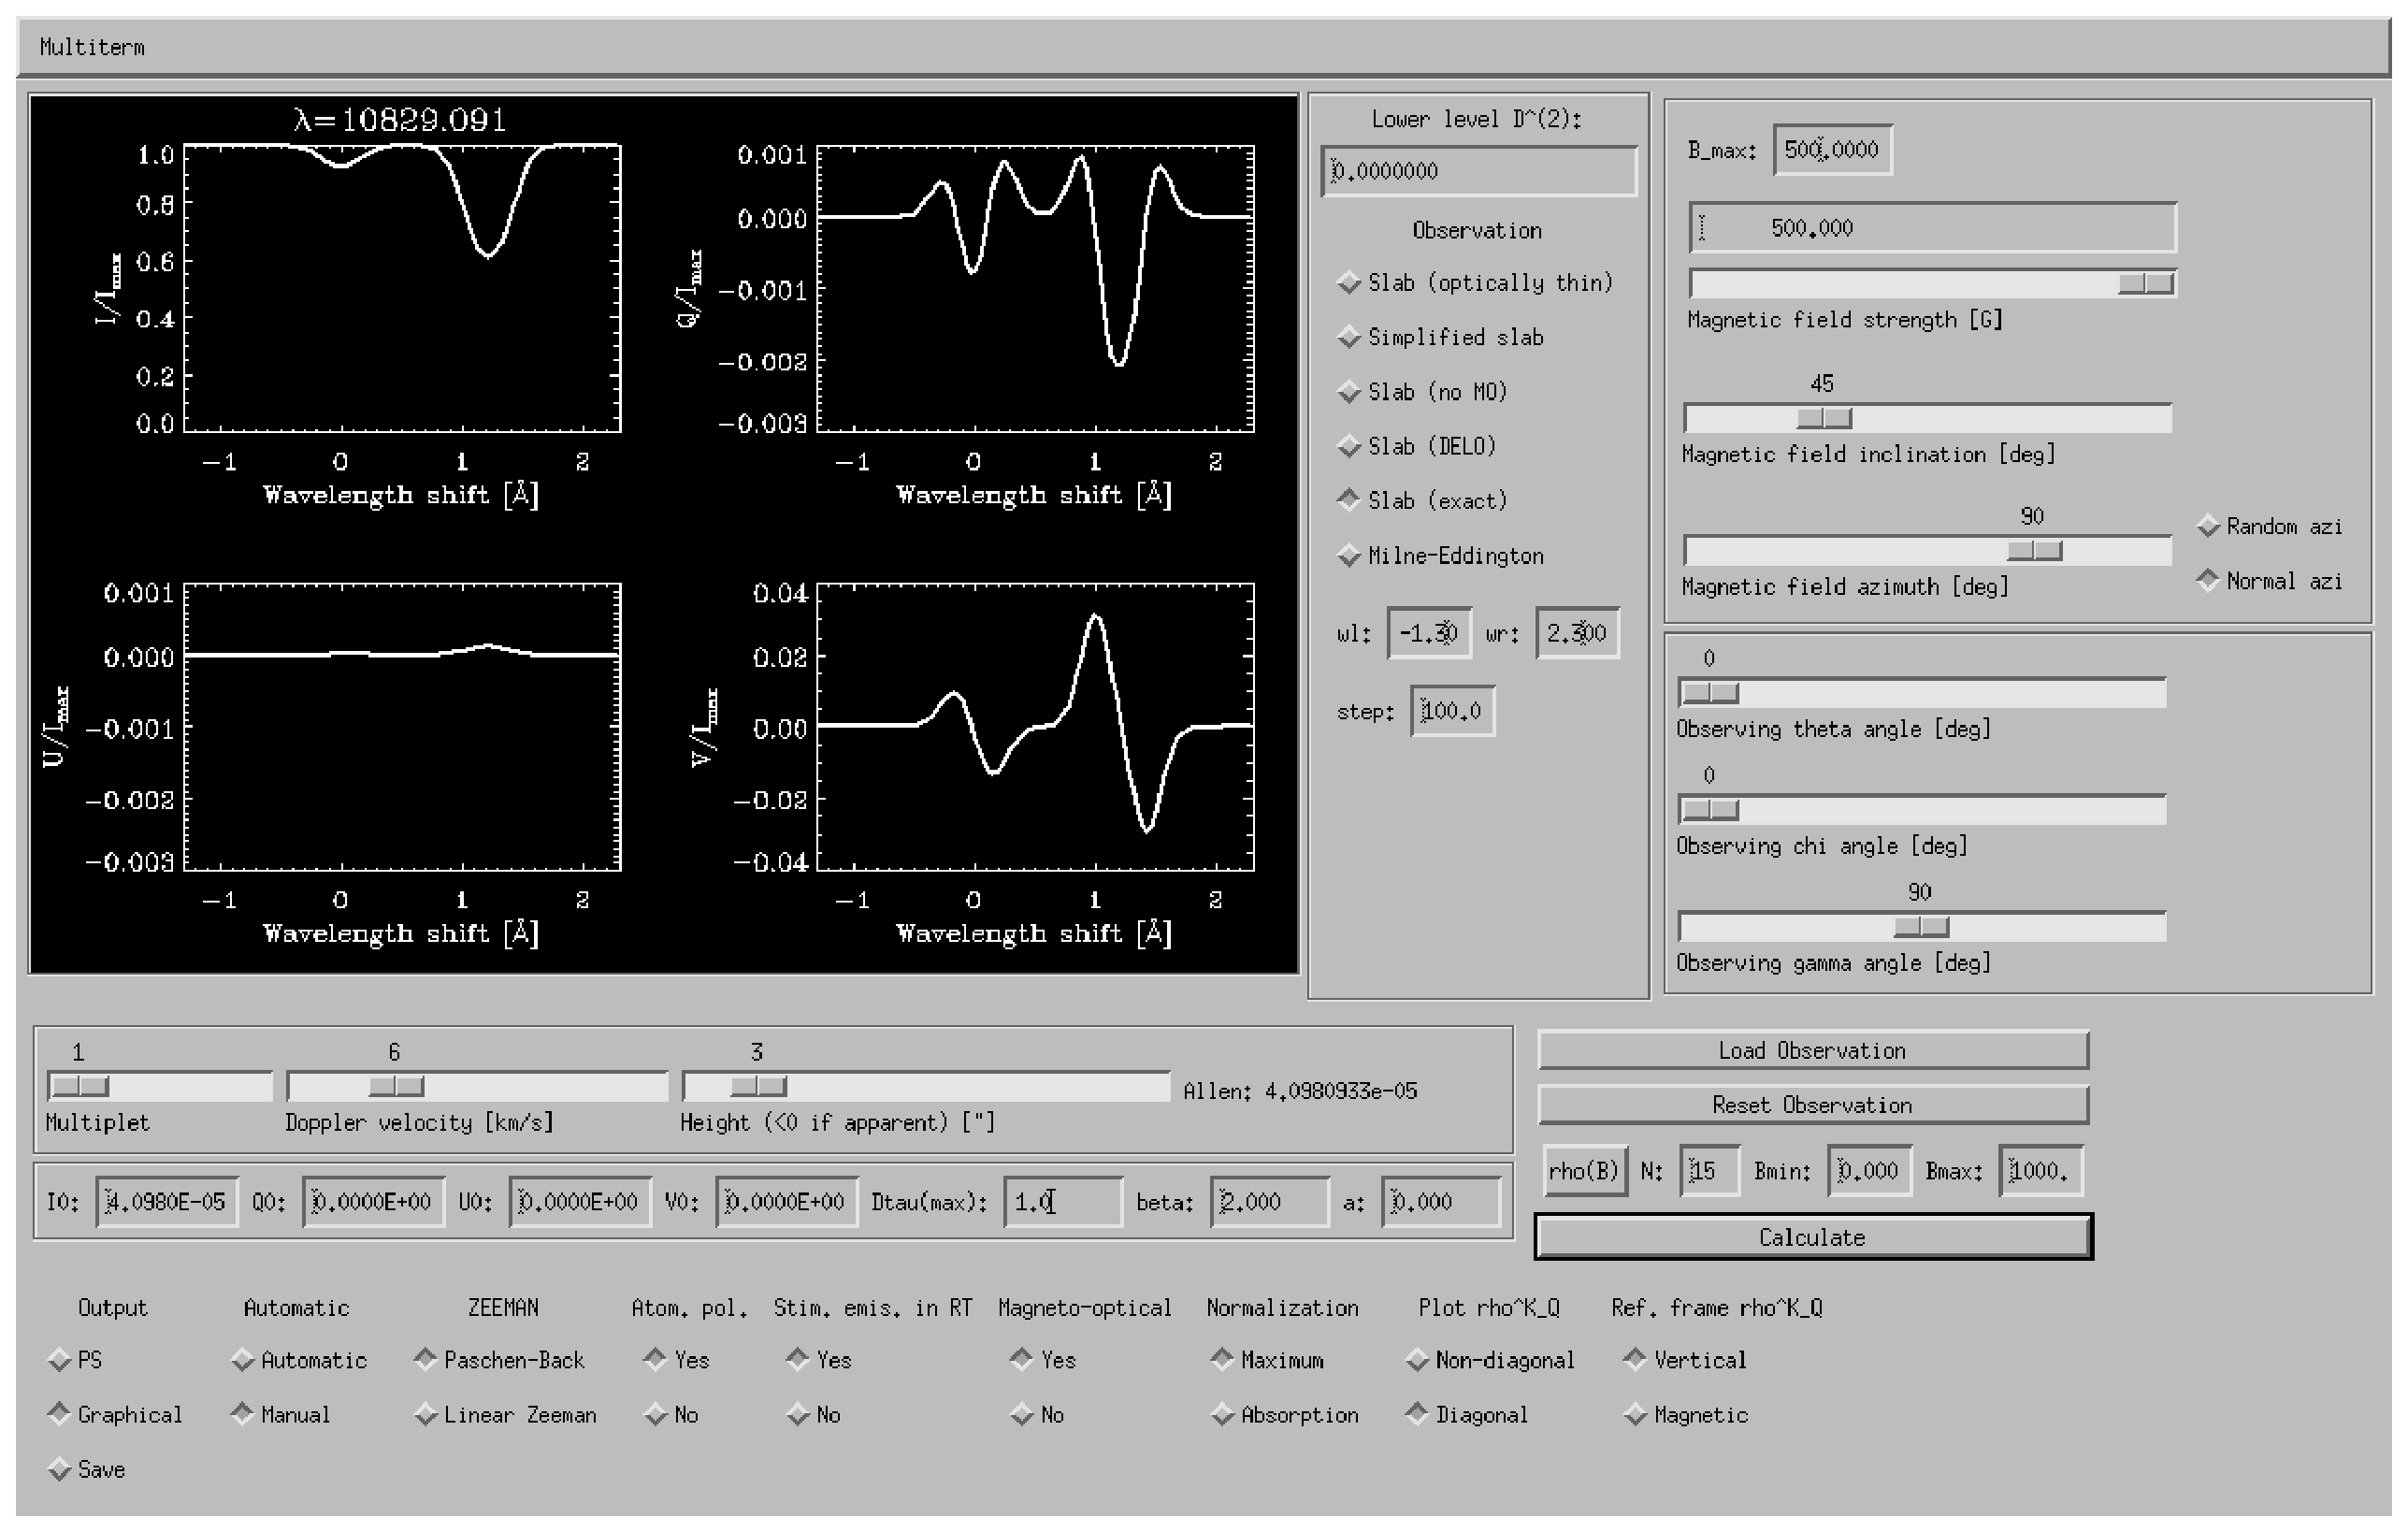
\includegraphics[width=\columnwidth]{f5.eps}
\caption{Screen dump of the graphical front-end used for the synthesis.
\label{fig:synthesis_GUI}}
\end{figure}

\section{Graphical front-ends}
Although the code can be run in command line by modifying by hand the input files, 
\H\ contains also two user friendly front-ends (GUI) for the simple execution and
analysis of the results. Note that the directory \texttt{IDL\_routines} has to be
in your IDL path.

\begin{figure}[!t]
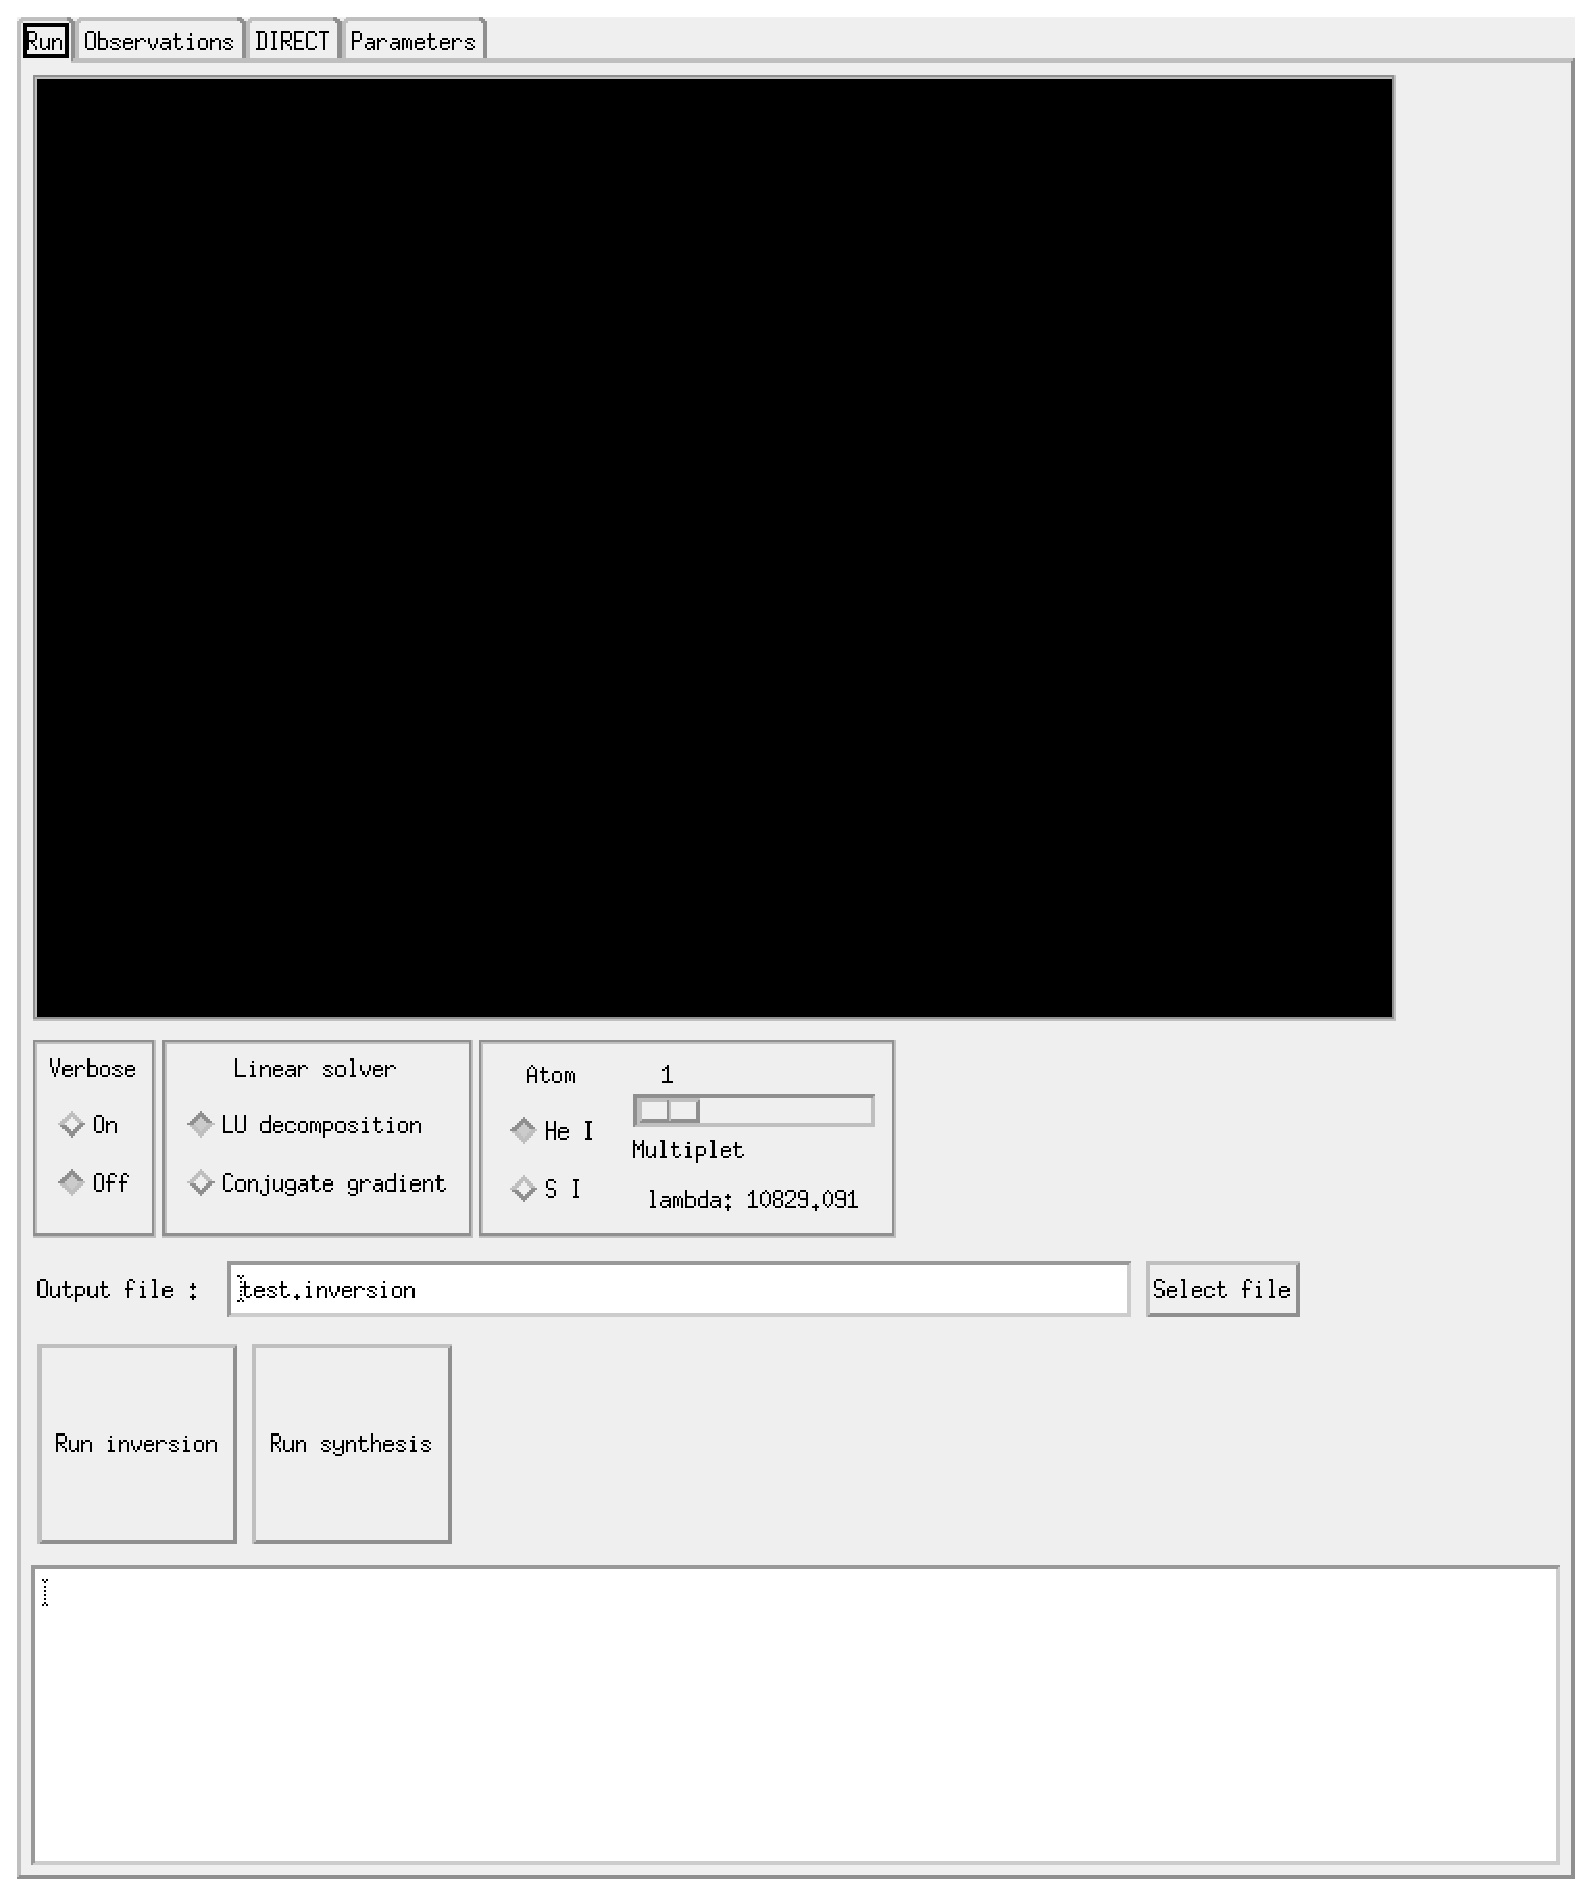
\includegraphics[width=0.48\columnwidth]{inv1.eps}%
\hspace{0.1cm}
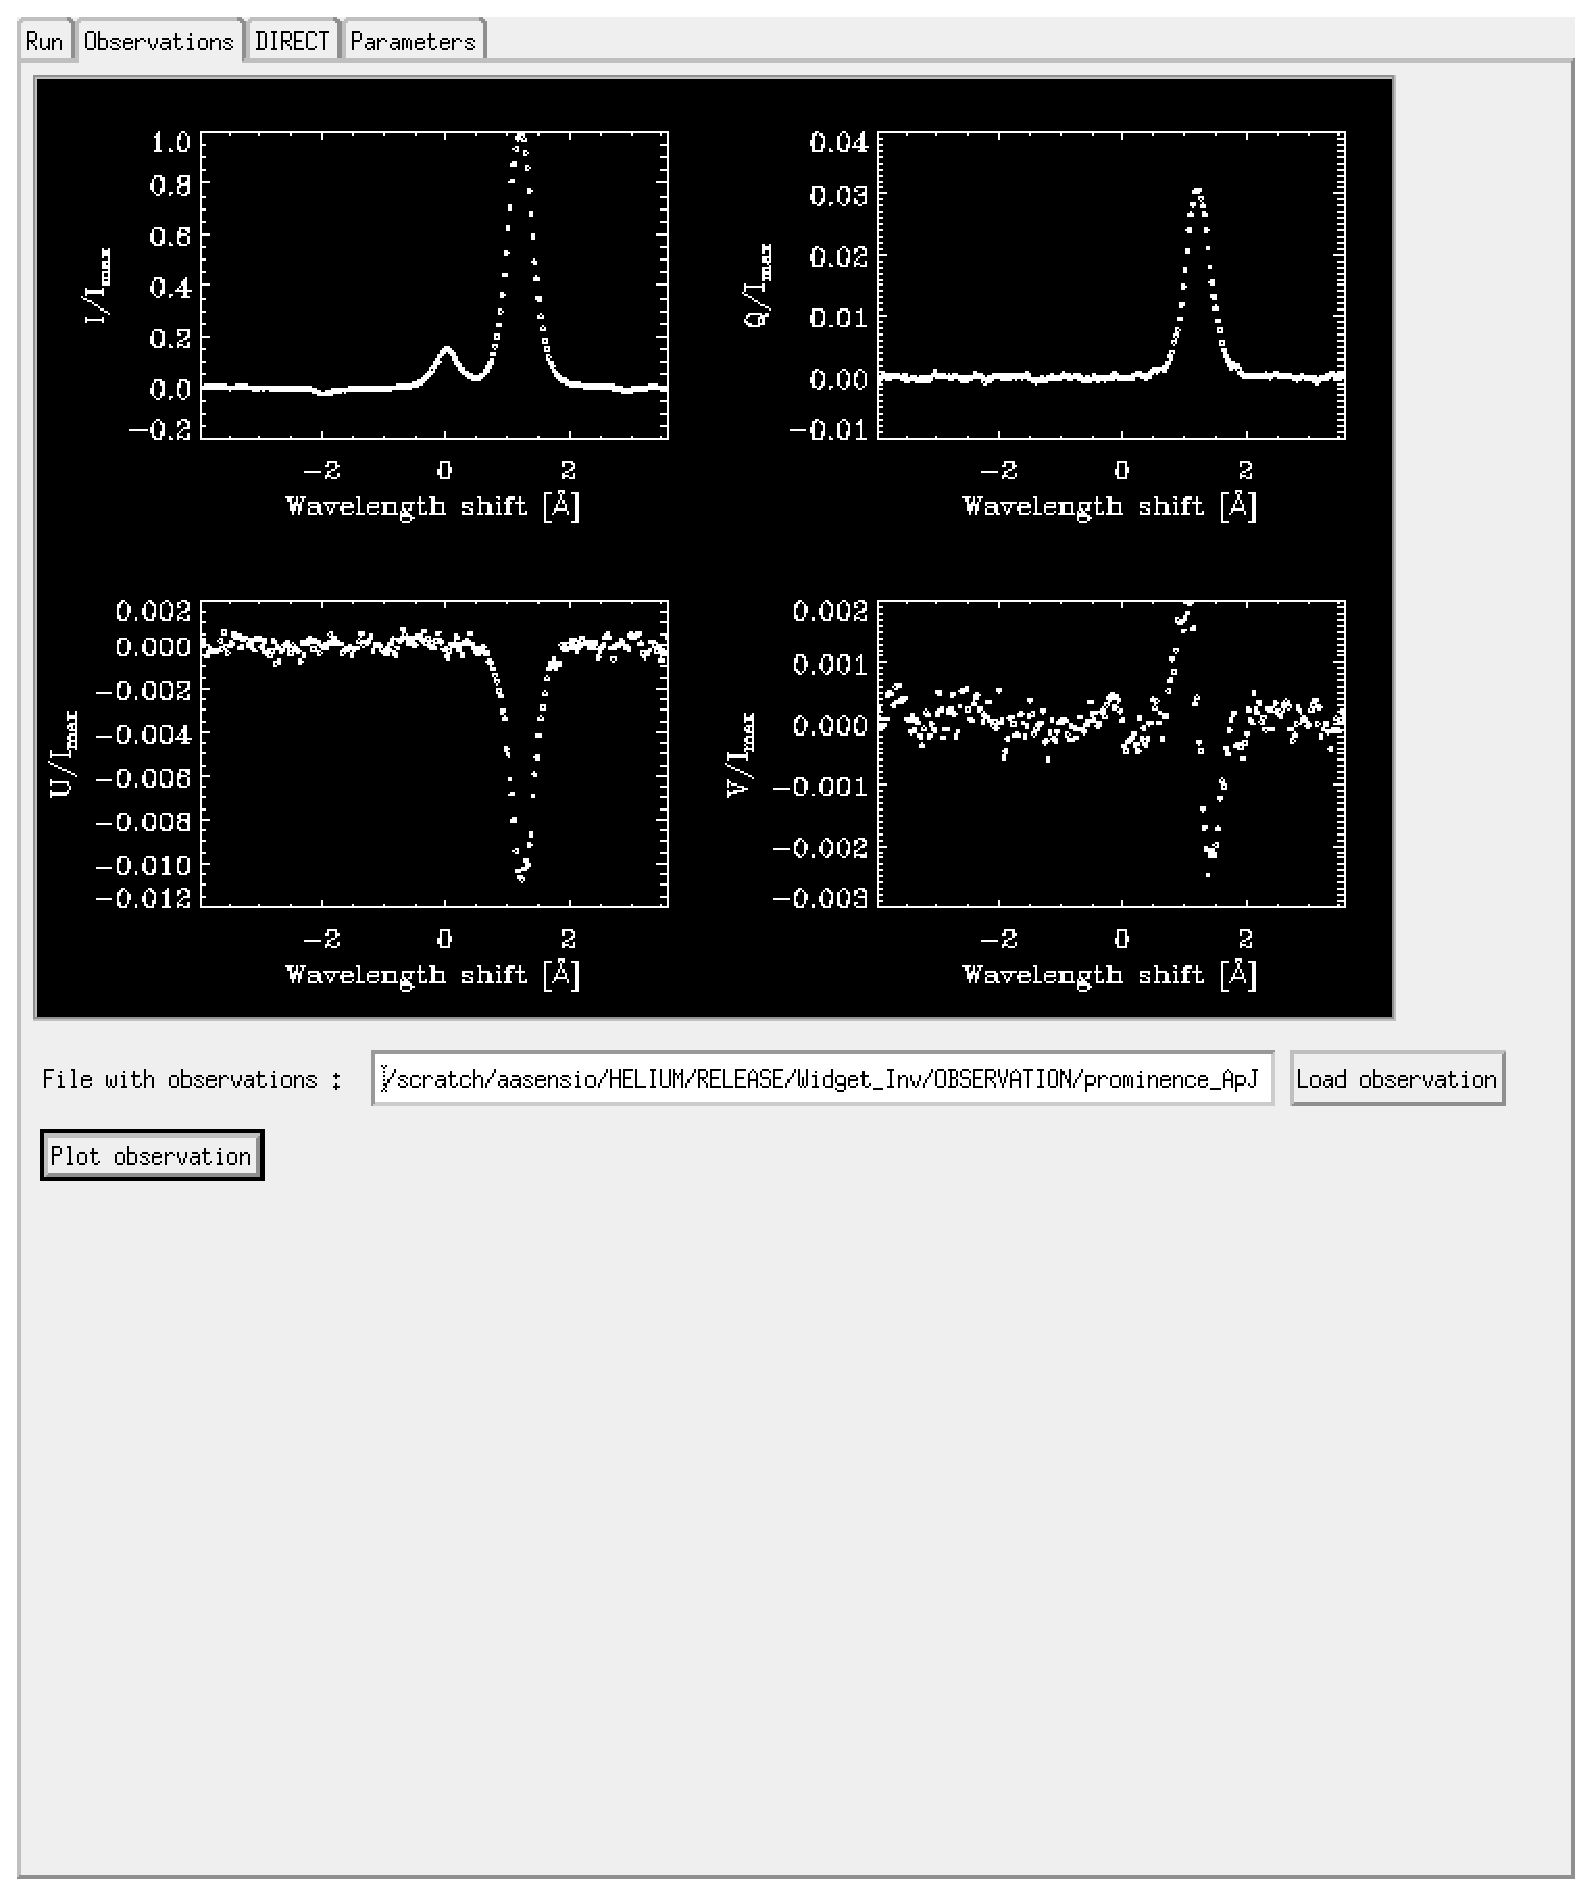
\includegraphics[width=0.48\columnwidth]{inv2.eps}
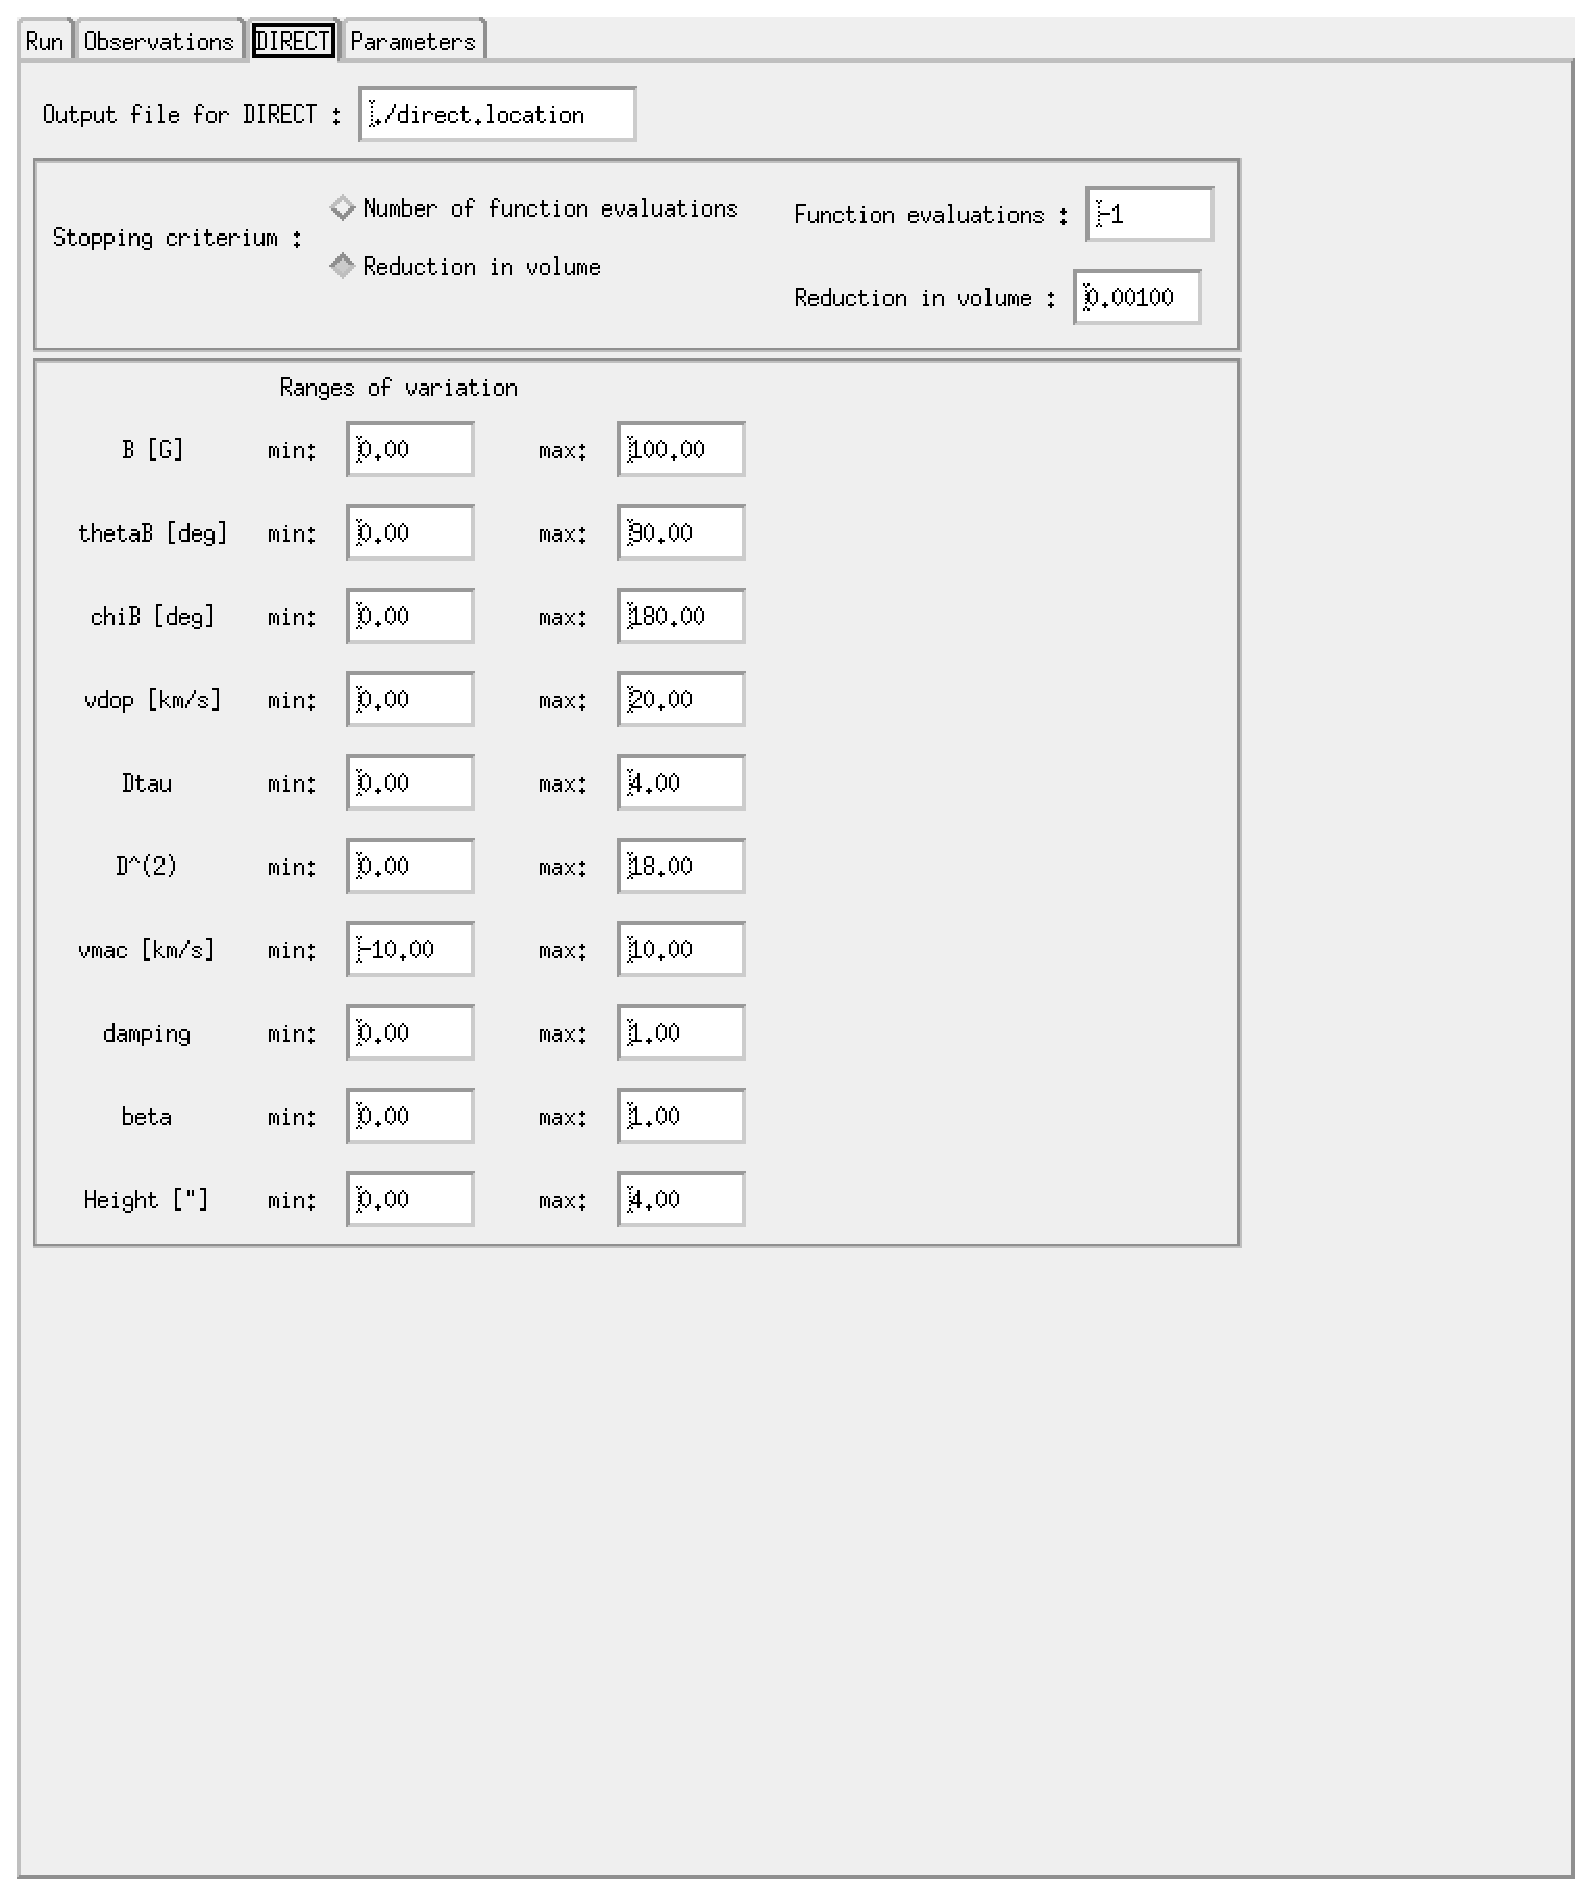
\includegraphics[width=0.48\columnwidth]{inv3.eps}%
\hspace{0.5cm}
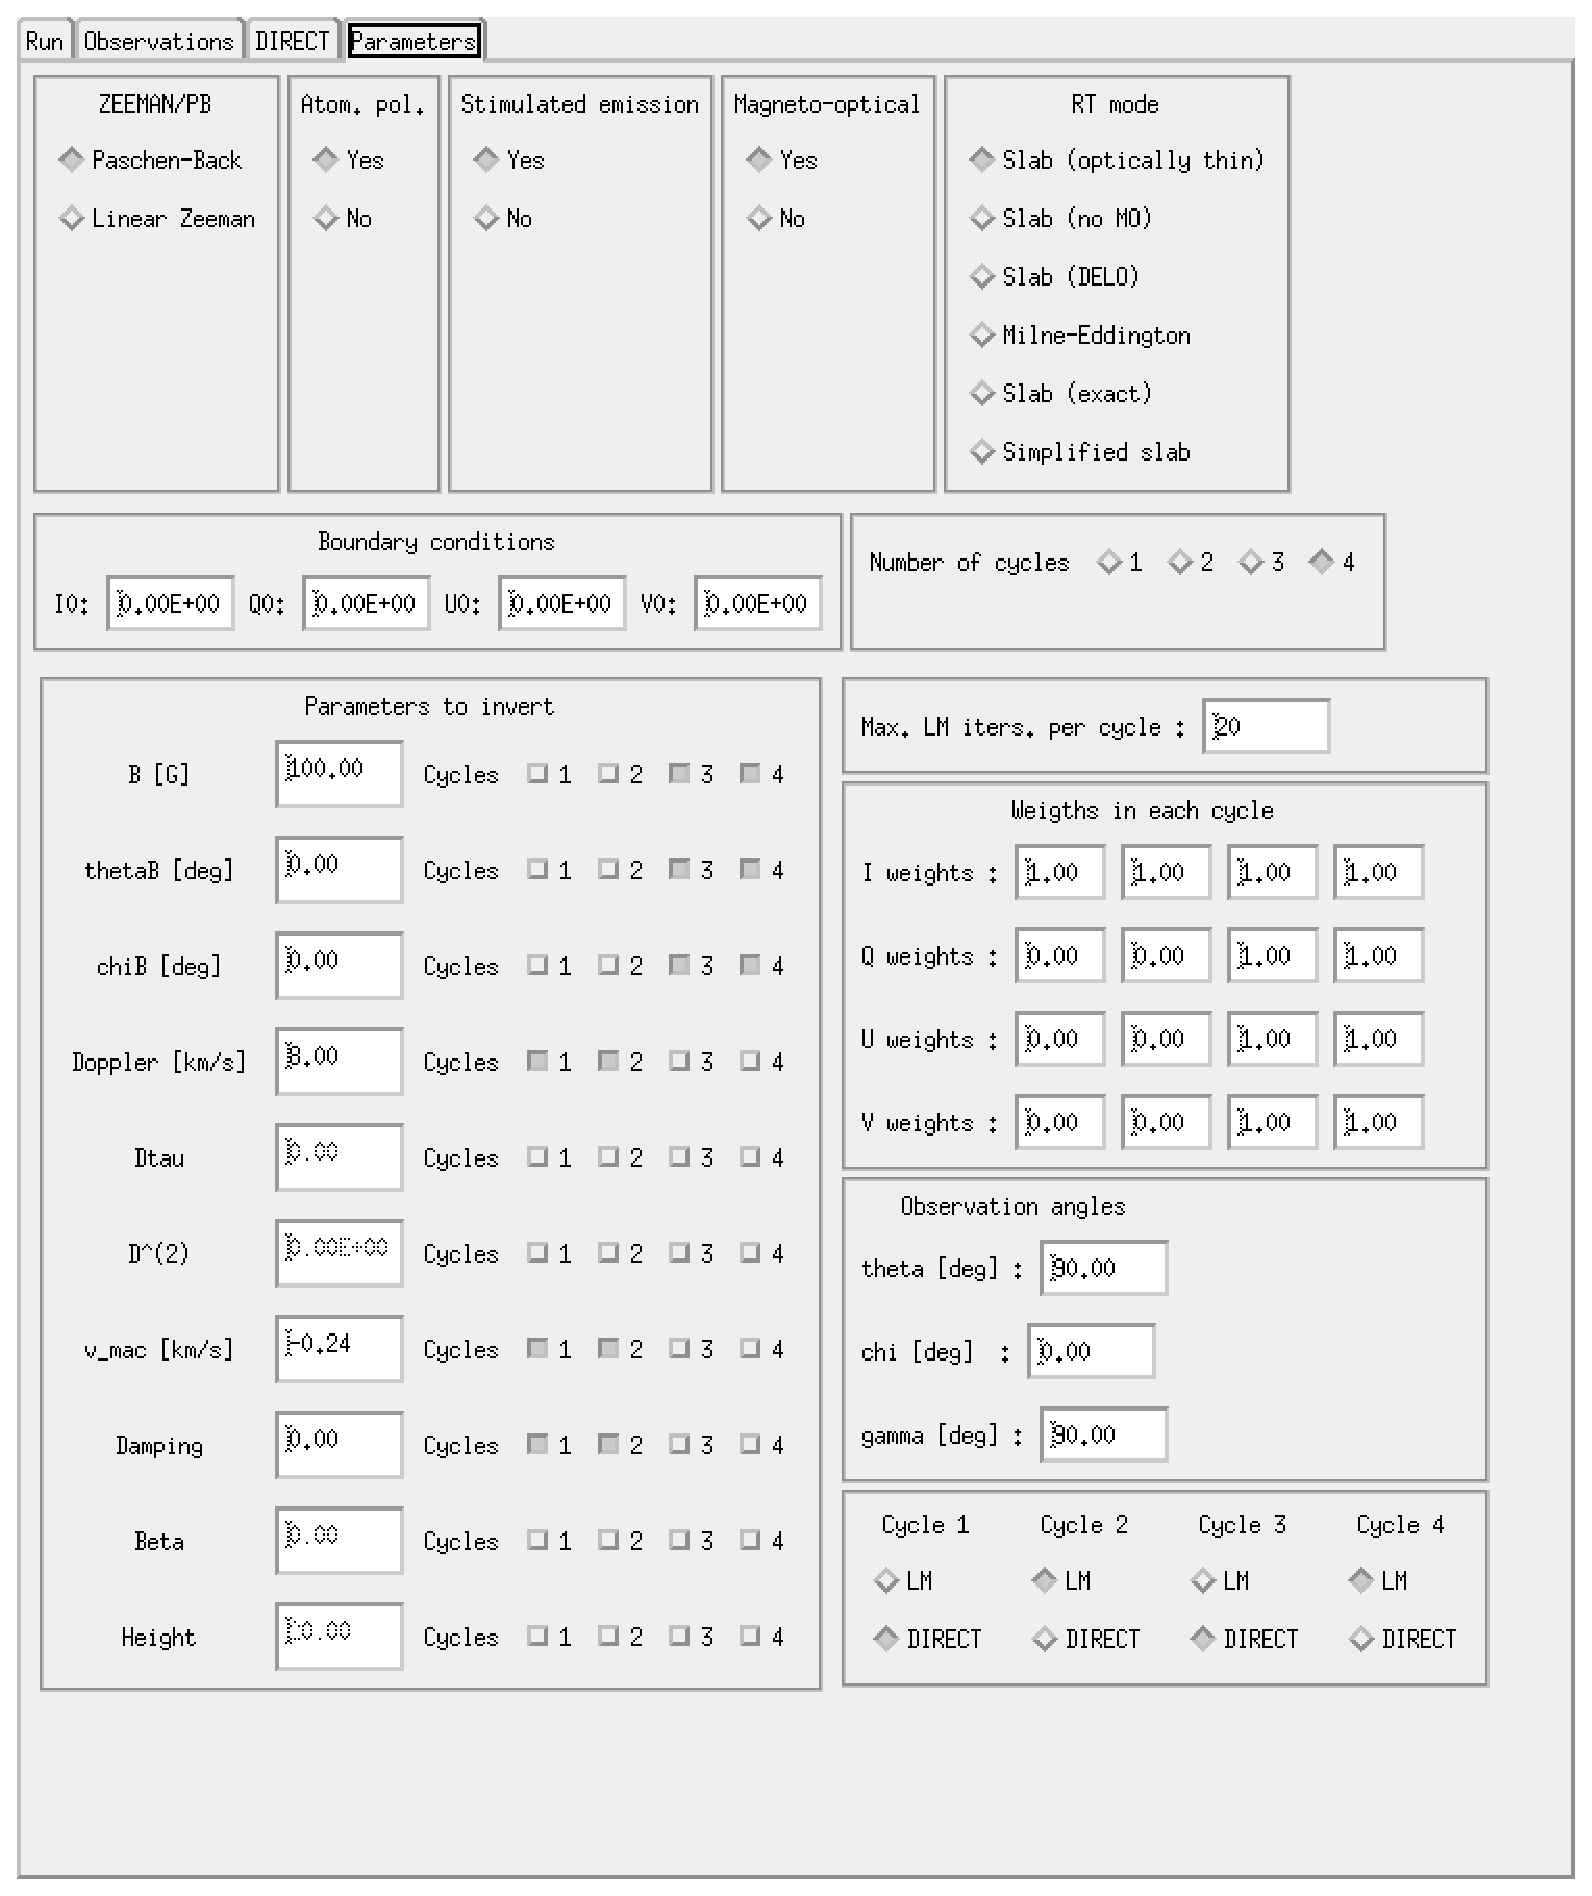
\includegraphics[width=0.48\columnwidth]{inv4.eps}
\caption{Screen dump of the graphical front-end used for the inversion.
\label{fig:inversion_GUI}}
\end{figure}


\subsection{Synthesis}
It is placed in the directory \texttt{Widget\_Synth} and it is invoked with the following commands:
\begin{verbatim}
IDL> .r hazel
IDL> hazel 
\end{verbatim}
Figure \ref{fig:synthesis_GUI} shows the GUI for the synthesis mode. All the parameters explained in
the previous sections (fundamentally those in \S\ref{sec:init_parameters}) are present in the
GUI. All the parameters are very simple to modify (when changing numerical values in the
GUI, always remember to press \texttt{Return} to activate the change) and clicking on \textbf{Calculate},
the window is updated with the new Stokes profiles.
The GUI also shows the value of the solar radiation field when the inclination of the line-of-sight
and the wavelength of the multiplet is changed. The value (which can be introduced in the
value of $I_0$ as a boundary condition) is given next to the height of the slab and
indicated with the label ``Allen''. In case of crashes, the GUI can be restarted with the following
command:
\begin{verbatim}
IDL> .r hazel
IDL> hazel, /reset
\end{verbatim}

\subsection{Inversion}
It is placed in the directory \texttt{Widget\_Inv} and it is invoked with the following commands:
\begin{verbatim}
IDL> .r hazel_inv
IDL> hazel_inv
\end{verbatim}
Again, in case of crashes, the GUI can be restarted with the following command:
\begin{verbatim}
IDL> .r hazel_inv
IDL> hazel_inv, /reset
\end{verbatim}
The GUI for the inversion is more complex because of the large amount of parameters that have
to be changed. For this reason, the GUI is composed of 4 pages, as indicated in 
Fig. \ref{fig:inversion_GUI}. 

The first page is used to select the output file, together with the 
atomic system and multiplet to be used. Finally, the button \textbf{Run inversion} will call
\H\ and update the state of the best model in the plot window.

The second page is used simply to load the file with the observed Stokes profile. A button
is also available to plot the observed data.

The third page controls the behavior of the DIRECT algorithm. It is essentially a graphical
representation of the \texttt{direct\_range.dat} file.

Finally, the fourth page controls the behavior of the cycles, the value of the fixed parameters,
the weights for each Stokes parameter and the level of physical realism introduced in the
simulation.

\section{\HM\ input/output files}
\label{sec:phazel_files}
Both input and output files for \HM\ are NetCDF files. 

\subsection{Input files}
The input file constains the
observations and information about the observing position and boundary condition. The file
consists of the following variables:
\begin{itemize}
\item lambda: vector of size \textit{nlambda} containing the wavelength axis with respect to the center of the multiplet.
\item map: array of size \textit{(npixel,8,nlambda)} containing the Stokes vector $(I,Q,U,V)$ and
the associated standard deviation of the noise $(\sigma_I,\sigma_Q,\sigma_U,\sigma_V)$.
\item boundary: array of size \textit{(npixel,4)} containing the boundary condition for every inverted pixel.
\item height: vector of size \textit{npixel} which contains the height of the slabs for every pixel.
\item obs\_theta: vector of size \textit{npixel} which contains the observing angle $\theta$ for every pixel.
\item obs\_gamma: vector of size \textit{npixel} which contains the observing angle $\gamma$ that defines the positive
reference for Stokes $Q$ for every pixel.
\item mask: array of size \textit{nx,ny} which tells whether this pixel will be inverted.
\item normalization: variable indicating whether the profiles are normalized to the peak amplitude or the continuum of Stokes $I$.
\item pars: array of size \textit{npixel,npars} which contains the initial value for the model parameters. These will be
used to reinvert some pixels or, for instance, to refine the ambiguous solutions.
\end{itemize}
The routine \texttt{gen\_netcdf.pro} on the directory \texttt{IDL\_routines} and the \texttt{genNetCDF.py} on \texttt{pyRoutines} shows functions that
generate such a file by passing all the variables as parameters.
The order of pars is the following, depending on the number of slabs:
\begin{itemize}
\item 1-component (vector of size 8): $B$, $\theta_B$, $\chi_B$, $\tau$, $v_\mathrm{dop}$, $a$, $v_\mathrm{mac}$, $\beta$
\item 2-component 1+1 with same field (vector of size 11): $B$, $\theta_B$, $\chi_B$, $\tau_1$, $\tau_2$, $v_\mathrm{dop}$, $a$, $v_\mathrm{mac1}$, $v_\mathrm{mac2}$, $\beta$, $\beta_2$
\item 2-component 1+1 with different field (vector of size 15): $B_1$, $\theta_{B1}$, $\chi_{B1}$, $B_2$, $\theta_{B2}$, $\chi_{B2}$, $\tau_1$, $\tau_2$, $v_\mathrm{dop}$, $v_\mathrm{dop2}$, $a$, $v_\mathrm{mac1}$, $v_\mathrm{mac2}$, $\beta$, $\beta_2$
\item 2-component 2 with different field with filling factor (vector of size 16): $B_1$, $\theta_{B1}$, $\chi_{B1}$, $B_2$, $\theta_{B2}$, $\chi_{B2}$, $\tau_1$, $\tau_2$, $v_\mathrm{dop}$, $v_\mathrm{dop2}$, $a$, $v_\mathrm{mac1}$, $v_\mathrm{mac2}$, $\mathrm{ff}$, $\beta$, $\beta_2$
\end{itemize}


\subsection{Output files}
The results of the inversion are saved on two files defined on the \texttt{config\_inversion.dat} configuration
file. The file with the inverted profiles contains the following variables:
\begin{itemize}
\item lambda: vector of size \textit{nlambda} containing the wavelength axis with respect to the center of the multiplet.
\item map: array of size \textit{(npixel,4,nlambda)} containing the synthetic Stokes vector $(I,Q,U,V)$ for every pixel.
\end{itemize}
The file with the inverted parameters contains the following variable:
\begin{itemize}
\item map: array of size \textit{(npixel,ncolumns)} containing the parameters of the inversion. 
\end{itemize}
The number of columns depends on the selected model:
\begin{itemize}
\item One-slab: nine columns with the vector $(B,\theta_B,\chi_B,h,\tau,v_\mathrm{th},a,v_\mathrm{mac},\beta)$.
\item Two-slab with same magnetic field: eleven columns with the vector \\ $(B,\theta_B,\chi_B,h,[\tau]_1,[\tau]_2,v_\mathrm{th},a,[v_\mathrm{mac}]_1,
[v_\mathrm{mac}]_2,\beta)$.
\item Two-slab with different magnetic field: fifteen columns with the vector \\ $([B]_1,[\theta_B]_1,[\chi_B]_1,[B]_2,[\theta_B]_2,[\chi_B]_2,
h,[\tau]_1,[\tau]_2,[v_\mathrm{th}]_1,[v_\mathrm{th}]_2,a,[v_\mathrm{mac}]_1,[v_\mathrm{mac}]_2,\beta)$.
\end{itemize}
The file \texttt{read\_results.pro} on the \texttt{RunMPI} directory shows how to read the
files from IDL.

\subsection{Ambiguities}
You have to remember that the results of Hazel are potentially affected by ambiguities and you have
to take them into account. There is an utility written in IDL that, given an inverted map, obtains
all the other solutions which are ambiguous in the saturation regime. This can be called, including the
appropriate paths and discarding the final \texttt{.nc} extension, by:
\begin{verbatim}
IDL> disamb, 'file_with_inversions', 'file_with_observations', angleObs
\end{verbatim}
where \texttt{angleObs} is the observation angle $\theta$ (so that it is 90$^\circ$ for an observation
exactly at the limb.
This program can be called with the additional \texttt{/gen\_files\_inversion}, which then generates
a set of observations, configuration files and a file to run \HM. This is useful in case the line is not
in the saturation regime. In this case, the ambiguous solutions that are found by the code are
not strictly valid and one should refine them with a final LM cycle in which $B$, $\theta_B$ and $\chi_B$
are left free. The solution to the ambiguities in the saturation regime is shown in Section \ref{sec:ambiguities}.

%%%%%%%%%%%%%%%%%%%%%%%%%%%%%%%%%%%%%%%%%%%%%%%%%%
%%%%%%%%%%%%%%%%%%%%%%%%%%%%%%%%%%%%%%%%%%%%%%%%%%
\section{Calling Hazel from Python}
We have developed a wrapper to allow the user to call the synthesis routines of Hazel in Python.
To do so, just enter into the directory \texttt{SourcePy} and type
\begin{verbatim}
python setup.py build_ext --inplace
\end{verbatim}
and a library \texttt{pyhazel.so} will be generated (and also copied to the directory
\texttt{RunPy}. In this very same directory you can see the \texttt{test.py} file that
shows how to call the code to wrapper.


%%%%%%%%%%%%%%%%%%%%%%%%%%%%%%%%%%%%%%%%%%%%%%%%%%
%%%%%%%%%%%%%%%%%%%%%%%%%%%%%%%%%%%%%%%%%%%%%%%%%%
\section{Basic Equations}
We consider a constant-property slab of atoms, located at a height
$h$ above the 
visible solar ``surface", in the presence of a deterministic magnetic field of
arbitrary strength $B$, 
inclination $\theta_B$ and azimuth $\chi_B$ (see Fig. 1). The slab's optical
thickness at the wavelength 
and line of sight under consideration is $\tau$.
We assume that all the atoms inside this slab are illuminated from below by the
photospheric solar continuum radiation field, whose center-to-limb variation has
been tabulated by \cite{pierce00}. The ensuing anisotropic radiation pumping
produces population imbalances and quantum coherences between pairs of magnetic
sublevels, even among those pertaining to the different $J$-levels of the
adopted atomic model. This atomic level polarization and the Zeeman-induced
wavelength shifts between the $\pi$ ($\Delta{M}=M_u-M_l=0$), $\sigma_{\rm blue}$
($\Delta{M}=+1$) and $\sigma_{\rm red}$ ($\Delta{M}=-1$) transitions produce
polarization in the emergent spectral line radiation.

In order to facilitate the understanding of the code, in 
the following we summarize the basic equations which allow us to 
calculate the spectral line polarization taking rigorously into account the 
joint action of atomic level polarization and the Hanle and Zeeman effects. To this end, we have applied the 
quantum theory of spectral line polarization, which is described in great detail 
in the monograph by \cite{landi_landolfi04}. We have also applied several methods 
of solution of the Stokes-vector transfer equation, some of which can be 
considered as particular cases of the two general methods explained in \S6 of \cite{trujillo03}.

\begin{figure}
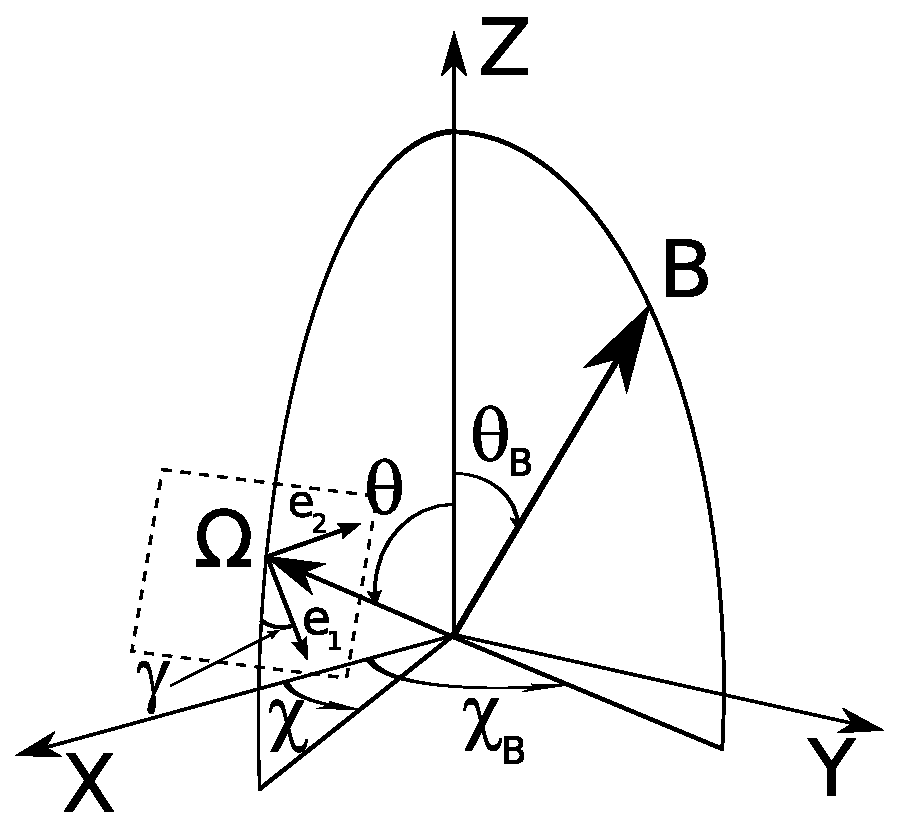
\includegraphics[width=\columnwidth]{f1.eps}
\caption{The geometry for the scattering event. The $Z$-axis is placed along the vertical
to the solar atmosphere. The magnetic field vector,
$\mathbf{B}$,
is characterized by its modulus $B$, the inclination angle $\theta_B$ and
the azimuth $\chi_B$. The line-of-sight, indicated by the unit vector
$\mathbf{\Omega}$,
is characterized by the two angles $\theta$ and $\chi$.
The reference direction for Stokes $Q$ is defined by the vector $\mathbf{e}_1$
on the plane
perpendicular to the line-of-sight. This vector makes an angle $\gamma$ with
respect to the plane formed by
the vertical and the line-of-sight. In the figures showing examples of the
emergent Stokes profiles, our
choice for the positive reference direction for Stokes $Q$ is $\gamma=90^\circ$, unless otherwise stated.
For off-limb observations, we have $\theta=90^\circ$, while for observations
on the solar disk, we have $\theta<90^\circ$. Note also that $\chi$ is generally taken to be $0^\circ$.
\label{fig:geometry}}
\end{figure}

\subsection{The radiative transfer approach}
\label{sec:radiative_transfer}
The emergent Stokes vector $\mathbf{I}(\nu,\mathbf{\Omega})=(I,Q,U,V)^{\dag}$
(with $\dag$=transpose, $\nu$ the frequency and $\mathbf{\Omega}$ the unit vector indicating 
the direction of propagation of the ray) is obtained by solving the radiative transfer equation

\begin{equation}
\frac{d}{ds}\mathbf{I}(\nu,\mathbf{\Omega}) =
\bm{\epsilon}(\nu,\mathbf{\Omega}) - \mathbf{K}(\nu,\mathbf{\Omega}) 
\mathbf{I}(\nu,\mathbf{\Omega}),
\label{eq:rad_transfer}
\end{equation}
where $s$ is the geometrical distance along the ray under consideration,
$\bm{\epsilon}(\nu,\mathbf{\Omega})=({\epsilon}_I,{\epsilon}_Q,{\epsilon
}_U,{\epsilon}_V)^{\dag}$ is the emission vector and
\begin{equation}
\mathbf{K} = \left( \begin{array}{cccc}
\eta_I & \eta_Q & \eta_U & \eta_V \\
\eta_Q & \eta_I & \rho_V & -\rho_U \\
\eta_U & -\rho_V & \eta_I & \rho_Q \\
\eta_V & \rho_U & -\rho_Q & \eta_I
\end{array} \right)
\label{eq:propagation}
\end{equation}
is the propagation matrix. Alternatively, introducing the optical distance along the ray,  
${\rm d}{\tau}=-{\eta_I}{\rm d}s$, one can write the Stokes-vector 
transfer Eq. (\ref{eq:rad_transfer}) in the following two ways:

\begin{itemize}

\item The first one, whose formal solution requires the use of the evolution operator introduced by \cite{landi_landi85}, is 
\begin{equation}
{{d}\over{d{\tau}}}{\bf I}\,=\,{\bf K}^{*}
{\bf I}\,-\,{\bf S}, 
\label{eq:rad_transfer_peo}
\end{equation}
where ${\bf K}^{*}={\bf K}/{\eta_I}$ and ${\bf S}=\bm{\epsilon}/{\eta_I}$. 
The formal solution of this equation can be seen in eq. (23) of \cite{trujillo03}.

\item The second one, whose formal solution does not require the use of the above-mentioned evolution operator is \citep[e.g.,][]{rees_delo89}
\begin{equation}
{{d}\over{d{\tau}}}{\bf I}\,=\,{\bf I}\,-\,{\bf S}_{\rm eff},  
\label{eq:rad_transfer_delo}
\end{equation}
where the effective source-function vector
$\,{\bf S}_{\rm eff}\,=\,{\bf S}\,-\,
{\bf K}^{'}{\bf I},\,\,\,$ being $\,{\bf K}^{'}={\bf K}^{*}-{\bf 1}$
(with $\bf 1$ the unit matrix). The formal solution of this equation can be seen in eq. (26) of \cite{trujillo03}.

\end{itemize}

Once
the coefficients $\epsilon_I$ and $\epsilon_X$ (with
$X=Q,U,V$) of the emission vector 
and the coefficients $\eta_I$, $\eta_X$, and
$\rho_X$ of the $4\times4$ propagation matrix are known 
at each point within the medium it is possible to solve formally Eq.
(\ref{eq:rad_transfer_peo}) or Eq.
(\ref{eq:rad_transfer_delo}) for
obtaining the emergent Stokes profiles for any desired line of sight.
Our computer program considers the following levels of sophistication for the solution of the radiative transfer equation: 

\begin{itemize}

\item {\em Numerical Solutions}.
The most general case, where the properties of the slab vary
along the ray path, has to be solved numerically. To this
end, two efficient and accurate methods of solution of 
the Stokes-vector transfer equation are those proposed by \cite{trujillo03} (see his eqs. (24) and (27), respectively). The starting points for the development of these two numerical methods were Eq. (\ref{eq:rad_transfer_peo}) and Eq. (\ref{eq:rad_transfer_delo}), respectively. Both methods can be considered as generalizations, to the Stokes-vector transfer case, of the well-known short characteristics method for the solution of the standard (scalar) transfer equation. 

\item {\em Exact analytical solution of the problem of a constant-property slab including the magneto-optical terms of the propagation matrix}. For the general case of a constant-property slab of arbitrary optical thickness we actually have the following analytical solution, which can be easily obtained as a particular case of eq. (24) of \cite{trujillo03}:

\begin{equation}
{\bf I}={\rm e}^{-{\mathbf{K}^{*}}\tau}\,{\bf I}_{\rm sun}\,+\,\left[{\mathbf{K}^{*}}\right]^{-1}\,
\left( \mathbf{1} - {\rm e}^{-{\mathbf{K}^{*}}\tau} \right) \,\mathbf{S},
\label{eq:slab_peo}
\end{equation}
where $\mathbf{I}_{\rm sun}$ is the Stokes
vector that illuminates the slab's boundary that is most distant from the
observer. We point out that the exponential of the propagation 
matrix ${\mathbf{K}^{*}}$ has an analytical expression similar to eq. (8.23) in \cite{landi_landolfi04}.

\item {\em Approximate analytical solution of the problem of a constant-property slab including the magneto-optical terms of the propagation matrix}. An approximate analytical solution to the constant-property slab problem can be easily obtained as a particular case of eq. (27) of \cite{trujillo03}:

\begin{equation}
\mathbf{I} = \left[ \mathbf{1}+\Psi_0 \mathbf{K}' \right]^{-1} \left[ \left(
e^{-\tau} \mathbf{1} - \Psi_M \mathbf{K}' \right) \mathbf{I}_{\rm sun} +
(\Psi_M+\Psi_0) \mathbf{S} \right],
\label{eq:slab_delo}
\end{equation}
where the coefficients $\Psi_M$ and $\Psi_0$ depend only on the optical thickness of the slab at the frequency and line-of-sight under consideration, since their expressions are:
\begin{eqnarray}
\Psi_M&=& \frac{1-e^{-\tau}}{\tau} - e^{-\tau},\nonumber \\
\Psi_0 &=&1-\frac{1-e^{-\tau}}{\tau}.
\end{eqnarray}

Note that Eq. (\ref{eq:slab_delo}) for the emergent Stokes vector is the one used by \cite{trujillo_asensio07} for 
investigating the impact of atomic level polarization on the Stokes profiles of the He {\sc i} 10830 \AA\ multiplet. 
We point out that, strictly speaking, it can be considered only as the exact analytical solution of the optically-thin 
constant-property slab problem\footnote{More precisely, when the optical thickness of the slab is small in comparison 
with the eigenvalues of the matrix $\mathbf{K}'$.}. The reason why Eq. (\ref{eq:slab_delo}) is, in general, an approximate 
expression for calculating the 
emergent Stokes vector is because  
its derivation assumes that the Stokes vector within the slab varies linearly with the optical distance. However, it provides 
a fairly good approximation to the emergent Stokes profiles (at least for all the problems we have investigated in this paper). 
Moreover, the results of fig. 2 of \cite{trujillo_asensio07} remain also virtually the same when using instead the exact 
Eq. (\ref{eq:slab_peo}), which from a computational viewpoint is significantly less efficient than the approximate Eq. (\ref{eq:slab_delo}).

\item {\em Exact analytical solution of the problem of a constant-property slab when neglecting the second-order terms of the Stokes-vector transfer equation}. Simplified expressions for the emergent Stokes vector can be obtained when 
$\epsilon_I{\gg}\epsilon_X$ and $\eta_I{\gg}(\eta_X,\rho_X)$, which justifies to neglect the second-order terms of Eq. (\ref{eq:rad_transfer}). The resulting approximate formulae for the emergent Stokes parameters are given by eqs. (9) and (10) of \cite{trujillo_asensio07}, which are identical to those used by \cite{trujillo_merenda05} for modeling the Stokes profiles observed in solar chromospheric spicules. We point out that there is a typing error in the sentence that introduces such eqs. (9) and (10) in \cite{trujillo_asensio07}, since they are obtained only when the above-mentioned second-order terms are neglected in Eq. (\ref{eq:rad_transfer}), although it is true that there are no magneto-optical terms in the resulting equations. 

\item {\em Optically thin limit}. Finally, the most simple solution 
is obtained when taking the optically thin limit ($\tau{\ll}1$) in the equations reported in the previous point, which lead to the equations (11) and (12) of \cite{trujillo_asensio07}. Note that if $\mathbf{I}_{\rm sun}=0$ (i.e., $I_0=X_0=0$), then such optically thin equations imply that ${X/I}\,{\approx}\,{\epsilon_X}/{\epsilon_I}$. 

\end{itemize}

The coefficients of the emission vector and of the propagation matrix
depend on the multipolar components, $\rho^K_Q(J,J^{'})$, of the atomic density
matrix. Let us recall now the meaning of these physical quantities and how to
calculate them in the presence of an arbitrary magnetic field under given
illumination conditions.  

%%%%%%%%%%%%%%%%%%%%%%%%%%%%%%%%%%%%%%%%
%%%%%%%%%%%%%%%%%%%%%%%%%%%%%%%%%%%%%%%%
\subsection{The multipolar components of the atomic density matrix}

We quantify the atomic polarization of the atomic levels using the multipolar components 
of the atomic density matrix. We assume that the atom can be correctly described under 
the framework of the $L$-$S$ coupling \citep[e.g.,][]{condon_shortley35}. The  
different $J$-levels are grouped in terms with well defined values of the
electronic angular momentum $L$ and the spin $S$. We neglect the influence of
hyperfine structure and assume that the energy
separation between the $J$-levels pertaining to 
each term is very small in comparison with the energy difference between
different terms. Therefore, we allow for coherences between
different 
$J$-levels pertaining to the same term but not between the $J$-levels
pertaining to 
different terms. As a result, we can represent the atom under the 
formalism of the multi-term atom discussed by \cite{landi_landolfi04}.

In the absence of magnetic fields the energy eigenvectors can be written using
Dirac's notation as $|\beta L S J M\rangle$, where
$\beta$ indicates a set of inner quantum numbers specifying the electronic
configuration. In general, if a magnetic field of 
arbitrary strength is present, the vectors $|\beta L S J M\rangle$ are no longer
eigenfunctions of the total Hamiltonian and $J$ is no longer a good quantum
number. In this
case, the eigenfunctions of the full Hamiltonian can be written as the following
linear combination:
\begin{equation}
\label{eq:eigenfunctions_total_hamiltonian}
|\beta L S j M\rangle = \sum_J C_J^j(\beta L S, M) |\beta L S J M\rangle,
\end{equation}
where $j$ is a pseudo-quantum number which is used for labeling the energy
eigenstates belonging to the subspace corresponding to assigned values of the
quantum numbers $\beta$, $L$, $S$, and $M$, and where the coefficients $C_J^j$
can be chosen to be real. 

In the presence of a magnetic field sufficiently weak so that the magnetic
energy is much smaller than the energy intervals between the $J$-levels, the energy eigenvectors are still
of the form $|\beta L S J M\rangle$ ($C_J^j(\beta L S, M) \approx \delta_{Jj}$), and the
splitting of the magnetic sublevels pertaining to each $J$-level is linear with the magnetic field strength. 
For stronger magnetic fields, we enter the incomplete Paschen-Back effect regime in which the energy eigenvectors are
of the general form given by Eq. (\ref{eq:eigenfunctions_total_hamiltonian}),
and the splitting among the various $M$-sublevels is no longer linear with the
magnetic strength. If the magnetic field strength is further increased we
eventually reach the so-called complete Paschen-Back effect regime, where the
energy eigenvectors are of the form $|L S M_L M_S\rangle$ and each $L$-$S$ term
splits into a number of components, each of which corresponding to particular
values of ($M_L+2M_S$).

Within the framework of the multi-term atom model the atomic polarization of the
energy levels is described with the
aid of the density matrix elements
\begin{equation}
\rho^{\beta L S}(jM,j'M') = \langle \beta L S j M | \rho | \beta L S j' M'\rangle,
\end{equation}
where $\rho$ is the atomic density matrix operator. Using the expression of the
eigenfunctions of the
total Hamiltonian given by Eq. (\ref{eq:eigenfunctions_total_hamiltonian}), the
density matrix 
elements can be rewritten as:
\begin{equation}
\rho^{\beta L S}(jM,j'M') = \sum_{JJ'} C_J^j(\beta L S, M) C_{J'}^{j'}(\beta L
S, M') \rho^{\beta L S}(JM,J'M'),
\end{equation}
where $\rho^{\beta L S}(JM,J'M')$ are the density matrix elements on the basis of
the eigenvectors $| \beta L S J M\rangle$.

Following \cite{landi_landolfi04}, it is helpful to use the spherical
statistical tensor 
representation, which is related to the previous one by the following linear
combination:
\begin{eqnarray}
{^{\beta LS}\rho^K_Q(J,J')} &=& \sum_{jj'MM'} C_J^j(\beta L S, M)
C_{J'}^{j'}(\beta L S, M') \nonumber \\
&\times& (-1)^{J-M} \sqrt{2K+1} \threej{J}{J'}{K}{M}{-M'}{-Q} 
\rho^{\beta L S}(jM,j'M'),
\end{eqnarray}
where the 3-j symbol is defined as indicated by any
suitable textbook on Racah algebra.

%%%%%%%%%%%%%%%%%%%%%%%%%%%%%%%%%%%%%%%%
%%%%%%%%%%%%%%%%%%%%%%%%%%%%%%%%%%%%%%%%
\subsection{Statistical equilibrium equations}
In order to obtain the
${^{\beta LS}\rho^K_Q(J,J')}$ elements we have to solve the  
statistical equilibrium equations. These equations, written in a reference
system in which 
the quantization axis ($Z$) 
is directed along the
magnetic field vector and
neglecting the 
influence of collisions, can be written as \citep{landi_landolfi04}:
\begin{eqnarray}
\frac{d}{dt} {^{\beta LS}\rho^K_Q(J,J')} &=& -2\pi \mathrm{i} \sum_{K' Q'}
\sum_{J'' J'''} N_{\beta LS}(KQJJ',K'Q'J''J''') {^{\beta LS}\rho^{K'}_{Q'}(J'',J''')}
\nonumber \\
&+& \sum_{\beta_\ell L_\ell K_\ell Q_\ell J_\ell J_\ell'} {^{\beta_\ell L_\ell
S}\rho^{K_\ell}_{Q_\ell}(J_\ell,J_\ell')} 
\mathbb{T}_A(\beta L S K Q J J', \beta_\ell L_\ell S K_\ell Q_\ell J_\ell
J_\ell') \nonumber \\
&+& \sum_{\beta_u L_u K_u Q_u J_u J_u'} {^{\beta_u L_u
S}\rho^{K_u}_{Q_u}(J_u,J_u')} 
\Big[ \mathbb{T}_E(\beta L S K Q J J', \beta_u L_u S K_u Q_u J_u J_u') \nonumber \\
& &\qquad \qquad \qquad \qquad \qquad + \mathbb{T}_S(\beta L S K Q
J J', \beta_u L_u S K_u Q_u J_u J_u') \Big] \nonumber \\
&-& \sum_{K' Q' J'' J'''} {^{\beta L S}\rho^{K'}_{Q'}(J'',J''') } \Big[
\mathbb{R}_A(\beta L S K Q J J' K' Q' J'' J''') \nonumber \\
& & + \mathbb{R}_E(\beta L S K Q J J' K'
Q' J'' J''') + \mathbb{R}_S(\beta L S K Q J J' K' Q' J'' J''') \Big].
\label{eq:see}
\end{eqnarray}
The first term in the right hand side of Eq. (\ref{eq:see}) takes into account
the 
influence of the magnetic field on the atomic level polarization. This term has 
its simplest expression in the chosen magnetic field
reference frame \citep[see eq. 7.41 of][]{landi_landolfi04}. 
In any other reference system, a more complicated expression
arises.
The second, third and fourth terms account, respectively, for coherence transfer due
to 
absorption from lower levels ($\mathbb{T}_A$), spontaneous emission from upper
levels 
($\mathbb{T}_E$) and stimulated emission from upper levels ($\mathbb{T}_S$).
The remaining terms account for the relaxation of coherences due to absorption to
upper 
levels ($\mathbb{R}_A$), spontaneous emission to lower levels ($\mathbb{R}_E$) 
and stimulated emission to lower levels ($\mathbb{R}_S$), respectively. 

The stimulated emission and absorption transfer and relaxation rates depend explicitly on 
the radiation field properties \citep[see eqs. 7.45 and 7.46 of][]{landi_landolfi04}.
The symmetry properties of the
radiation 
field are accounted for by the spherical components of the radiation field
tensor:

\begin{equation}
J^K_Q(\nu) = \oint \frac{d\Omega}{4\pi} \sum_{i=0}^3
\mathcal{T}^K_Q(i,\mathbf{\Omega}) S_i(\nu,\mathbf{\Omega}).
\label{eq:jkq}
\end{equation}
The quantities $\mathcal{T}^K_Q(i,\mathbf{\Omega})$ are spherical tensors that
depend
on the reference frame and on the  
ray direction $\mathbf{\Omega}$. They are given by
\begin{equation}
\mathcal{T}^K_Q(i,\mathbf{\Omega}) = \sum_P t^K_P(i) \mathcal{D}^K_{PQ}(R'),
\label{eq:tkq}
\end{equation}
where $R'$ is the rotation that carries the reference system defined by
the line-of-sight $\mathbf{\Omega}$ and by the polarization unit vectors $\mathbf{e}_1$ and
$\mathbf{e}_2$ into the reference system of the magnetic field, 
while $\mathcal{D}^K_{PQ}(R')$
is the usual rotation matrix \citep[e.g.,][]{edmonds60}.
Table 5.6 in \cite{landi_landolfi04} gives the
$\mathcal{T}^K_Q(i,\mathbf{\Omega})$ values for each Stokes parameter $S_i$ (with $S_0=I$, $S_1=Q$, $S_2=U$ and $S_3=V$).

%%%%%%%%%%%%%%%%%%%%%%%%%%%%%%%%%%%%%%%%
%%%%%%%%%%%%%%%%%%%%%%%%%%%%%%%%%%%%%%%%
\subsection{Emission and absorption coefficients}
Once the multipolar components ${^{\beta L S}\rho^{K}_{Q}(J,J') }$ are known, the
coefficients $\epsilon_I$ and $\epsilon_X$ (with
$X=Q,U,V$) of the emission vector 
and the coefficients $\eta_I$, $\eta_X$, and
$\rho_X$ of the propagation matrix
for a given transition between an upper 
term $(\beta L_u S)$ and an lower term $(\beta L_\ell S)$ can be
calculated with the expressions of \S7.6.b in  
\cite{landi_landolfi04}. 
These radiative transfer coefficients are proportional to the number density of \ion{He}{1} atoms, $\mathcal{N}$. Their defining expressions contain also the Voigt profile and the Faraday-Voigt profile \citep[see \S5.4 in][]{landi_landolfi04}, which involve the following parameters: $a$ (i.e., the reduced damping constant), $v_\mathrm{th}$ (i.e., the velocity  that characterizes the thermal motions, which
broaden the line profiles), and $v_\mathrm{mac}$ (i.e., the velocity of possible bulk motions in the plasma, which produce a Doppler shift). 

It is important to emphasize that the expressions for 
the emission and absorption coefficients and those of the statistical
equilibrium equations are written in the reference system whose quantization
axis is parallel to the magnetic field. The following equation indicates how to
obtain the density matrix elements in a new reference system:
\begin{equation}
\left[ {^{\beta L S}\rho^{K}_{Q}(J,J') } \right]_\mathrm{new} = \sum_{Q'} \left[
{^{\beta L S}\rho^{K}_{Q'}(J,J') } \right]_\mathrm{old}
\mathcal{D}^K_{Q' Q}(R)^*,
\end{equation}
where $\mathcal{D}^K_{Q' Q}(R)^*$ is the complex conjugate of the rotation matrix for the rotation $R$ that carries the 
old reference system into the new one.


%%%%%%%%%%%%%%%%%%%%%%%%%%%%%%%%%%%%%%%%
%%%%%%%%%%%%%%%%%%%%%%%%%%%%%%%%%%%%%%%%

\section{Inversion}
Our inversion strategy is based on the minimization of a merit function 
that quantifies how well the Stokes profiles calculated in our atmospheric model
reproduce the observed Stokes
profiles. To this end, we have 
chosen the standard $\chi^2$--function, defined as:
\begin{equation}
\chi^2 = \frac{1}{4N_\lambda} \sum_{i=1}^4 \sum_{j=1}^{N_\lambda} 
\frac{\left[S_i^\mathrm{syn}(\lambda_j)-S_i^\mathrm{obs}(\lambda_j) \right]^2}{
\sigma_i^2(\lambda_j)} ,
\end{equation}
where $N_\lambda$ is the number of wavelength points and $\sigma_i^2(\lambda_j)$ is the
variance associated to the $j$-th wavelength point of the $i$-th Stokes profiles. The minimization 
algorithm tries to find the value of the parameters of our model that lead to
synthetic Stokes profiles $S_i^\mathrm{syn}$ with the best possible fit to the 
observations. 
For our slab model, the number of
parameters (number of dimensions of the $\chi^2$ hypersurface) lies between 5
and
7, the maximum value corresponding to the optically thick case. 
The magnetic field vector 
($B$, $\theta_B$ and $\chi_B$), the thermal velocity ($v_\mathrm{th}$) and the
macroscopic velocity ($v_\mathrm{mac}$) are always required. This set of
parameters is enough 
for the case of an optically thin slab. In order to account for radiative
transfer 
effects, we need to define the optical depth of the slab along its normal
direction and at a suitable
reference wavelength (e.g., the central wavelength of the red blended component
for the \ion{He}{1} 10830 \AA\ multiplet). In addition, 
we may additionally need to include the damping parameter ($a$) of the Voigt profile if
the wings of the observed Stokes profiles cannot be fitted 
using Gaussian line profiles.


%%%%%%%%%%%%%%%%%%%%%%%%%%%%%%%%%%%%%%%%
%%%%%%%%%%%%%%%%%%%%%%%%%%%%%%%%%%%%%%%%
\subsection{Global Optimization techniques}
In order to avoid the possibility of getting trapped in a local minimum of the
$\chi^2$ hypersurface, global 
optimization methods have to be used. 
We have chosen the DIRECT algorithm 
\citep{Jones_DIRECT93}, whose name derives from one of its main 
features: \emph{di}viding \emph{rect}angles. The idea is to recursively sample 
parts of the space of parameters, improving in each iteration the location of
the part of the space 
where the global minimum is potentially located. The decision algorithm is based
on the assumption that the function is Lipschitz continuous \citep[see][for details]{Jones_DIRECT93}.
The method works very well in practice and can indeed find the minimum in 
functions that do not fulfill the condition of Lipschitz continuity. The reason
is that the DIRECT algorithm does not require the explicit calculation of the 
Lipschitz constant but it uses all possible values of such a constant to determine
if a region of the parameter space should be broken into subregions because of
its potential interest \citep[see][for details]{Jones_DIRECT93}. 

Since the 
intensity profile is not very sensitive to
the presence of a magnetic field (at least for magnetic field 
strengths of the order of or smaller than 1000 G), we have decided to estimate
the optical
thickness of the slab, the thermal and the macroscopic velocity of the
plasma and the damping constant by using only the Stokes $I$ profile, and then to determine the magnetic
field
vector by using the polarization profiles. 
The full inversion scheme
begins by applying the DIRECT method to obtain a first estimation of the
indicated four
parameters by using only Stokes $I$.  Afterwards, 
some LM iterations are carried out to refine the initial values of the  
model's parameters obtained in the previous step. Once the LM method 
has converged, the inferred values of $v_\mathrm{th}$, $v_\mathrm{mac}$ 
(together with $a$ and $\Delta \tau$, when these are parameters of the model)
are kept fixed in the next steps, 
in which the DIRECT method is used again for obtaining an initial approximation
of 
the magnetic field vector 
($B$,$\theta_B$,$\chi_B$). 
According to our experience,
the first estimate of the magnetic field vector given by the DIRECT algorithm 
is typically very close to the final solution. Nevertheless, some iterations of
the LM method are performed to refine the value of the magnetic field strength,
inclination and azimuth.
In any case, although we have found very good results with this procedure, the
specific inversion scheme
is fully configurable and can be tuned for specific problems.

Our experience has proved that the following strategy is appropriate for inverting
prominences. Two initial DIRECT+LM cycles with weights $(1,0,0,0)$ to
invert the thermodynamical parameters. Then, two DIRECT+LM cycles in which $B$, $\theta_B$
and $\chi_B$ are left free with weights $(0,0.1,0.1,1)$ which tries to set the
correct polarity of the field given by Stokes $V$. An additional LM cycle in which
we fit only $\theta_B$ and $\chi_B$ with the weights $(0,1,1,0.3)$ and a last
LM cycle with weights $(0,0.3,0.3,1)$ leaving the full magnetic field vector free.


%%%%%%%%%%%%%%%%%%%%%%%%%%%%%%%%%%%%%%%%
%%%%%%%%%%%%%%%%%%%%%%%%%%%%%%%%%%%%%%%%
\subsection{Convergence}
\label{sec:convergence}
We let the DIRECT algorithm
locate the global minimum in a region whose hypervolume is $V$. This hypervolume is 
obtained as the product of the length $d_i$ of each dimension associated with
each of the $N$ parameters:
\begin{equation}
V = \prod_i^N d_i.
\end{equation}
When the hypervolume decreases by a factor $f$ after the DIRECT algorithm
has discarded some of the hyperrectangles, its size along each dimension is
approximately decreased by a factor $f^{1/N}$. 
In order to end up with a small region
where the global minimum is located, many subdivisions are 
necessary, thus requiring many function evaluations. 

The most time consuming part of any optimization procedure is the evaluation of
the merit function. The DIRECT algorithm needs only a reduced number of evaluations 
of the merit function to find
the region where the global minimum is located. For this reason, we have
chosen it as the initialization part of the LM method. Since the initialization
point is close to the global minimum, the LM method, thanks to its quadratic behavior,
rapidly converges to the minimum.

\subsection{Stopping criterium}
We have used two stopping criteria for the
DIRECT algorithm. The first one is stopping when the ratio between the
hypervolume where
the global minimum is located and the original hypervolume is smaller than a
given threshold.
This method has been chosen when using the DIRECT 
algorithm as an initialization for the LM method, giving very good results. The
other good
option, suggested by \cite{Jones_DIRECT93}, is to stop after a fixed number of
evaluations of the merit function.  

%%%%%%%%%%%%%%%%%%%%%%%%%%%%%%%%%%%%%%%%%%%%%%%%%%%%%%%%%%%%%%%%%%%%%%%%%%%%%%%%%%%%%%%%%%%%%
%%%%%%%%%%%%%%%%%%%%%%%%%%%%%%%%%%%%%%%%%%%%%%%%%%%%%%%%%%%%%%%%%%%%%%%%%%%%%%%%%%%%%%%%%%%%%
\section{Ambiguities in the Hanle effect in the saturation regime}
\label{sec:ambiguities}
%%%%%%%%%%%%%%%%%%%%%%%%%%%%%%%%%%%%%%%%%%%%%%%%%%%%%%%%%%%%%%%%%%%%%%%%%%%%%%%%%%%%%%%%%%%%%
%%%%%%%%%%%%%%%%%%%%%%%%%%%%%%%%%%%%%%%%%%%%%%%%%%%%%%%%%%%%%%%%%%%%%%%%%%%%%%%%%%%%%%%%%%%%%
In the saturation regime of the Hanle effect, Stokes $Q$ and $U$ are insensitive to the field
strength, but are sensitive to the geometry of the field. For a $J=0 \to J=1$ transition, the linear
polarization can be written as:
\begin{eqnarray}
Q &=& \frac{q}{2} \left( 3 \cos^2 \theta_B-1 \right) \sin^2\Theta_B \cos 2\Phi_B \nonumber \\
U &=& \frac{q}{2} \left( 3 \cos^2 \theta_B-1 \right) \sin^2\Theta_B \sin 2\Phi_B.
\end{eqnarray}
These expressions contain a mixture of angles to make it clear that the polarization amplitude
depends on both the angle between the vertical and the magnetic field and between the magnetic
field and the line-of-sight (LOS).

The coordinates of the magnetic field vector $\mathbf{B}$ in the reference system of the vertical
and the reference system of the LOS are:
\begin{eqnarray}
\mathbf{B} &=& B \left(\sin \theta_B \cos \phi_B \mathbf{i}+\sin \theta_B \sin \phi_B \mathbf{j}+\cos \theta_B \mathbf{k} \right) \nonumber \\
\mathbf{B} &=& B \left(\sin \Theta_B \cos \Phi_B \mathbf{i}'+\sin \Theta_B \sin \Phi_B \mathbf{j}'+\cos \Theta_B \mathbf{k}' \right),
\end{eqnarray}
where the unit vectors are related by a simple rotation:
\begin{eqnarray}
\mathbf{i}' &=& \cos \theta \mathbf{i} - \sin \theta \mathbf{k} \nonumber \\
\mathbf{k}' &=& \sin \theta \mathbf{i} + \cos \theta \mathbf{k}.
\end{eqnarray}
Introducing these relations on the expression for the magnetic field, we find that the
following has to be fulfilled, given that the magnetic field vector is the same in both reference systems:
\begin{eqnarray}
\sin \theta_B \cos \phi_B &=& \sin \Theta_B \cos \Phi_B \cos \theta + \cos \Theta_B + \sin \theta \nonumber \\
\sin \theta_B \sin \phi_B &=& \sin \Theta_B \sin \Phi_B \nonumber \\
\cos \theta_B &=& \cos \Theta_B \cos \theta - \sin \Theta_B \cos \Phi_B \sin \theta.
\end{eqnarray}
Solving the previous three equations in the two directions, we find the following transformations
between the angles in the vertical reference system and the LOS reference system:
\begin{eqnarray}
\cos \Theta_B &=& \cos\theta \cos\theta_B + \sin\theta \sin\theta_B \cos\phi_B \nonumber \\
\sin \Theta_B &=& +\sqrt{1-\cos^2\Theta_B} \nonumber \\
\cos \Phi_B &=& \frac{\cos\theta \sin\theta_B \cos\phi_B - \cos\theta_B \sin\theta}{\sin \Theta_B} \nonumber \\
\sin \Phi_B &=& \frac{\sin\theta_B \sin\phi_B}{\sin\Theta_B}
\end{eqnarray}
and
\begin{eqnarray}
\cos \theta_B &=& \cos\theta \cos\Theta_B - \sin\theta \sin\Theta_B \cos\Phi_B \nonumber \\
\sin \theta_B &=& +\sqrt{1-\cos^2\theta_B} \nonumber \\
\cos \phi_B &=& \frac{\cos\theta \sin\Theta_B \cos\Phi_B + \cos\Theta_B \sin\theta}{\sin \theta_B} \nonumber \\
\sin \phi_B &=& \frac{\sin\Theta_B \sin\Phi_B}{\sin\theta_B}.
\end{eqnarray}
Note that, since $\Theta_B \in [0,\pi]$, we can safely use the square root and take the positive value.
In order to transform from one reference system to the other, we can compute the
inclination easily by inverting the sinus or the cosinus. However, the situation is different
for the azimuth, because the range of variation is $[-\pi,\pi]$. Therefore, one has to compute the 
cosinus and the sinus separately and the decide which is the correct quadrant fo the angle in terms
of the signs of both quantities.

% \begin{center}
% \input{figure_geometry}
% \end{center}

Four possible kinds of ambiguities can exist for the Stokes $Q$ and $U$ parameters. The idea is that $\Phi_B$
can be modified and still obtain the same $Q$ and $U$ by properly adjusting the value of $\Theta_B$. It is
clear that, given that the term that can be used to compensate for the change in the azimuth on the LOS
reference system is the same for Stokes $Q$ and $U$, we can only compensate for changes in the sign. Therefore,
we have the following potential ambiguities:
\begin{eqnarray}
\Phi_B' &=& \Phi_B \nonumber \\
\Phi_B' &=& \Phi_B -\pi/2 \nonumber \\
\Phi_B' &=& \Phi_B + \pi/2 \nonumber \\
\Phi_B' &=& \Phi_B + \pi.
\end{eqnarray}
For each case, we have to compute the value of $\Theta_B'$ that keeps the value of $Q$ and $U$ unchanged. Therefore,
once we find a solution to the inversion problem in the form of the pair $(\theta_B,\phi_B)$, we can find
the remaining solutions in the saturation regime following the recipes that we present now. Remember that, unless
one knows the polarity of the field, or in other words, the sign $\cos\Theta_B$, the number of potential
ambiguous solutions is 8. If the polarity of the field is known, the number is typically reduced to 4 (or 2
if no 90$^\circ$ ambiguity is present).

\section{\texorpdfstring{$\Phi_B' = \Phi_B$}{PhiB'=PhiB}}
Under this change, we have that
\begin{equation}
\cos 2\Phi_B' = \cos 2\Phi_B, \quad \sin 2\Phi_B' = \sin 2\Phi_B, \quad \cos \Phi_B' = \cos \Phi_B, \quad \sin \Phi_B' = \sin \Phi_B.
\end{equation}
Making use of the previous relations between the angles wrt to the vertical and the LOS, we have to solve the 
following equation:
\begin{equation}
\left( 3 \cos^2\theta_B'-1 \right) \sin^2 \Theta_B' = \left( 3 \cos^2\theta_B-1 \right) \sin^2 \Theta_B,
\end{equation}
which can be written as:
\begin{equation}
\left[ 3 \left( \cos \Theta_B' \cos \theta - \sin\theta \sin\Theta_B' \cos\Phi_B\right)^2-1 \right] \sin^2 \Theta_B' = 
\left[ 3 \left( \cos \Theta_B \cos \theta - \sin\theta \sin\Theta_B \cos\Phi_B\right)^2-1 \right] \sin^2 \Theta_B.
\end{equation}
After some algebra and doing the substitution $t=\sin\Theta_B'$, we end up with the following equation to be
solved:
\begin{equation}
A t^4 + Bt^2 + C t^3 \sqrt{1-t^2} = K,
\end{equation}
where
\begin{eqnarray}
A &=& -3\cos^2 \theta + 3\sin^2 \theta \cos^2 \Phi_B \nonumber \\
B &=& 3\cos^2 \theta - 1 \nonumber \\
C &=& -6 \cos\theta \sin\theta \cos \Phi_B \nonumber \\
K &=& \left[ 3 \left( \cos \Theta_B \cos \theta - \sin\theta \sin\Theta_B \cos\Phi_B\right)^2-1 \right] \sin^2 \Theta_B.
\end{eqnarray}
The previous equation can be solved if we make the change of variables $t=\pm \sqrt{Z}$, resulting in:
\begin{equation}
(C^2+A^2) Z^4 + (-C^2+2AB) Z^3 + (-2AK+B^2) Z^2 - 2BKZ + K^2 = 0.
\end{equation}
This polynomial of 4-th order can have four different solutions. From these solutions, we have to take only
the real solutions which are larger than 0, given the range of variation of $\Theta_B$:
\begin{equation}
t \in \mathbb{R}, \qquad 0 \leq t \leq 1.
\end{equation}
Once the solutions for $t$ are found, we make $\Theta_B' = \arcsin t$. Note that, for a fixed value of $t$,
two values of $\Theta_B'$ are possible. We choose the correct one by evaluating the expressions for 
$Q$ and $U$ and testing which of the two possible choices give the values equal (or very similar) to the original ones.

The angles $(\theta_B,\phi_B)$ are obtained by doing the transformation from $(\Theta_B',\Phi_B)$ to the
vertical reference system.

\section{\texorpdfstring{$\Phi_B' = \Phi_B+\pi$}{PhiB'=PhiB+pi}}
Under this change, we have:
\begin{equation}
\cos 2\Phi_B' = \cos 2\Phi_B, \quad \sin 2\Phi_B' = \sin 2\Phi_B, \quad \cos \Phi_B' = -\cos \Phi_B, \quad \sin \Phi_B' = -\sin \Phi_B.
\end{equation}
Following the same approach, we have to solve for $\Theta_B'$ in 
\begin{equation}
\left[ 3 \left( \cos \Theta_B' \cos \theta + \sin\theta \sin\Theta_B' \cos\Phi_B\right)^2-1 \right] \sin^2 \Theta_B' = 
\left[ 3 \left( \cos \Theta_B \cos \theta - \sin\theta \sin\Theta_B \cos\Phi_B\right)^2-1 \right] \sin^2 \Theta_B.
\end{equation}
The solution are obtained as the roots of the same equations as before but now
\begin{eqnarray}
A &=& -3\cos^2 \theta + 3\sin^2 \theta \cos^2 \Phi_B \nonumber \\
B &=& 3\cos^2 \theta - 1 \nonumber \\
C &=& 6 \cos\theta \sin\theta \cos \Phi_B \nonumber \\
K &=& \left[ 3 \left( \cos \Theta_B \cos \theta - \sin\theta \sin\Theta_B \cos\Phi_B\right)^2-1 \right] \sin^2 \Theta_B.
\end{eqnarray}

The angles $(\theta_B,\phi_B)$ are obtained by doing the transformation from $(\Theta_B',\Phi_B+\pi)$ to the
vertical reference system.

\section{\texorpdfstring{$\Phi_B' = \Phi_B+\pi/2$}{PhiB'=PhiB+pi/2}}
Under this change, we have:
\begin{equation}
\cos 2\Phi_B' = -\cos 2\Phi_B, \quad \sin 2\Phi_B' = -\sin 2\Phi_B, \quad \cos \Phi_B' = -\sin \Phi_B, \quad \sin \Phi_B' = \cos \Phi_B.
\end{equation}
Following the same approach, we have to solve for $\Theta_B'$ in 
\begin{equation}
\left[ 3 \left( \cos \Theta_B' \cos \theta + \sin\theta \sin\Theta_B' \sin\Phi_B\right)^2-1 \right] \sin^2 \Theta_B' = 
\left[ 3 \left( \cos \Theta_B \cos \theta - \sin\theta \sin\Theta_B \cos\Phi_B\right)^2-1 \right] \sin^2 \Theta_B.
\end{equation}
The solution are obtained as the roots of the same equations as before but now
\begin{eqnarray}
A &=& -3\cos^2 \theta + 3\sin^2 \theta \sin^2 \Phi_B \nonumber \\
B &=& 3\cos^2 \theta - 1 \nonumber \\
C &=& 6 \cos\theta \sin\theta \sin \Phi_B \nonumber \\
K &=& -\left[ 3 \left( \cos \Theta_B \cos \theta - \sin\theta \sin\Theta_B \cos\Phi_B\right)^2-1 \right] \sin^2 \Theta_B.
\end{eqnarray}

The angles $(\theta_B,\phi_B)$ are obtained by doing the transformation from $(\Theta_B',\Phi_B+\pi/2)$ to the
vertical reference system.


\section{\texorpdfstring{$\Phi_B' = \Phi_B-\pi/2$}{PhiB'=PhiB-pi/2}}
Under this change, we have:
\begin{equation}
\cos 2\Phi_B' = -\cos 2\Phi_B, \quad \sin 2\Phi_B' = -\sin 2\Phi_B, \quad \cos \Phi_B' = \sin \Phi_B, \quad \sin \Phi_B' = -\cos \Phi_B.
\end{equation}
Following the same approach, we have to solve for $\Theta_B'$ in 
\begin{equation}
\left[ 3 \left( \cos \Theta_B' \cos \theta + \sin\theta \sin\Theta_B' \sin\Phi_B\right)^2-1 \right] \sin^2 \Theta_B' = 
\left[ 3 \left( \cos \Theta_B \cos \theta - \sin\theta \sin\Theta_B \cos\Phi_B\right)^2-1 \right] \sin^2 \Theta_B.
\end{equation}
The solution are obtained as the roots of the same equations as before but now
\begin{eqnarray}
A &=& -3\cos^2 \theta + 3\sin^2 \theta \sin^2 \Phi_B \nonumber \\
B &=& 3\cos^2 \theta - 1 \nonumber \\
C &=& -6 \cos\theta \sin\theta \sin \Phi_B \nonumber \\
K &=& -\left[ 3 \left( \cos \Theta_B \cos \theta - \sin\theta \sin\Theta_B \cos\Phi_B\right)^2-1 \right] \sin^2 \Theta_B.
\end{eqnarray}

The angles $(\theta_B,\phi_B)$ are obtained by doing the transformation from $(\Theta_B',\Phi_B-\pi/2)$ to the
vertical reference system.


\section*{Acknowledgements}
We would like to thank Egidio Landi Degl'Innocenti and Marco Landolfi
for sharing with us their deep knowledge on the physics of the spectral line polarization,
which they have described in great detail in their
rigorous monograph on ``Polarization in Spectral Lines". Finantial support by 
the Spanish Ministry of Education and Science through projects AYA2007-63881 and 
the European Commission through the SOLAIRE network (MTRN-CT-2006-035484) is gratefully acknowledged.


\bibliographystyle{apj}
% \bibliography{apjmnemonic,/scratch/Dropbox/biblio}

\begin{thebibliography}{11}
\expandafter\ifx\csname natexlab\endcsname\relax\def\natexlab#1{#1}\fi

\bibitem[{{Belluzzi} {et~al.}(2007){Belluzzi}, {Trujillo Bueno}, \& {Landi
  Degl'Innocenti}}]{belluzzi07}
{Belluzzi}, L., {Trujillo Bueno}, J., \& {Landi Degl'Innocenti}, E. 2007, ApJ,
  666, 588

\bibitem[{{Condon} \& {Shortley}(1935)}]{condon_shortley35}
{Condon}, E.~U., \& {Shortley}, G.~H. 1935, The Theory of Atomic Spectra
  (Cambridge: Cambridge University Press)

\bibitem[{{Edmonds}(1960)}]{edmonds60}
{Edmonds}, A.~R. 1960, Angular Momentum in Quantum Mechanics (Princeton
  University Press)

\bibitem[{{Jones} {et~al.}(1993){Jones}, {Perttunen}, \&
  {Stuckmann}}]{Jones_DIRECT93}
{Jones}, D.~R., {Perttunen}, C.~D., \& {Stuckmann}, B.~E. 1993, Journal of
  Optimization Theory and Applications, 79, 157

\bibitem[{{Landi Deglinnocenti} \& {Landi Deglinnocenti}(1985)}]{landi_landi85}
{Landi Deglinnocenti}, E., \& {Landi Deglinnocenti}, M. 1985, Sol. Phys., 97,
  239

\bibitem[{{Landi Degl'Innocenti} \& {Landolfi}(2004)}]{landi_landolfi04}
{Landi Degl'Innocenti}, E., \& {Landolfi}, M. 2004, Polarization in Spectral
  Lines (Kluwer Academic Publishers)

\bibitem[{{Pierce}(2000)}]{pierce00}
{Pierce}, K. 2000, in Allen's Astrophysical Quantities, ed. A. N. Cox (New
  York: Springer Verlag and AIP Press)

\bibitem[{{Rees} {et~al.}(1989){Rees}, {Durrant}, \& {Murphy}}]{rees_delo89}
{Rees}, D.~E., {Durrant}, C.~J., \& {Murphy}, G.~A. 1989, ApJ, 339, 1093

\bibitem[{{Trujillo Bueno}(2003)}]{trujillo03}
{Trujillo Bueno}, J. 2003, in Stellar Atmosphere Modeling, ed. I.~{Hubeny},
  D.~{Mihalas}, \& K.~{Werner}, ASP Conf. Ser. 288 (San Francisco: ASP), 551

\bibitem[{{Trujillo Bueno} \& {Asensio Ramos}(2007)}]{trujillo_asensio07}
{Trujillo Bueno}, J., \& {Asensio Ramos}, A. 2007, ApJ, 655, 642

\bibitem[{{Trujillo Bueno} {et~al.}(2005){Trujillo Bueno}, {Merenda},
  {Centeno}, {Collados}, \& {Landi Degl'Innocenti}}]{trujillo_merenda05}
{Trujillo Bueno}, J., {Merenda}, L., {Centeno}, R., {Collados}, M., \& {Landi
  Degl'Innocenti}, E. 2005, ApJ, 619, L191

\end{thebibliography}


\end{document}
